% Two side to save paper
% openrigth means to put the chapter tittle on the right pages 
\documentclass[12pt,letterpaper,twoside,openright]{book}

\usepackage[spanish]{babel}
\usepackage[utf8]{inputenc}

% We define some strings that will use along
\def \thesiskeywords {}
\def \pdfauthor {Ricardo Román}
\def \thesistitle {Modelo de sensibilidad de los parámetros de frecuencia de la Transformada de Trazo para la clasificación de imágenes aéreas}

\usepackage[bookmarks=true, linktoc=all, colorlinks=false, pdftitle={\thesistitle}, pdfauthor={\pdfauthor}, pdfsubject={\thesistitle}, pdfkeywords={\thesiskeywords}, linkcolor=blue,filecolor=blue,urlcolor=blue,citecolor=blue]{hyperref}

%\usepackage{apacite}
%\let\APAbibcite\bibcite
\bibliographystyle{ieeetr}



\usepackage{epigraph}
\usepackage{acronym}
\usepackage{fancyhdr}
\usepackage{mdwlist}
\usepackage{alltt}
\usepackage{setspace}
\usepackage[pdftex]{graphicx}
\usepackage[scaled]{helvet} % ss
\usepackage{courier} % tt
\usepackage[T1]{fontenc}
\usepackage{indentfirst}
\usepackage{amsmath}
\usepackage{longtable}
\usepackage{siunitx}
%\usepackage{lib/algorithm-es}
\usepackage{algorithm}
\usepackage{caption}
\usepackage{subfigure}
\usepackage[hmargin={3.5cm,2.5cm},vmargin=2.5cm]{geometry}
\usepackage{enumitem}
\setlist{nosep} % or \setlist{noitemsep} to leave space around whole list

\usepackage{color}
\definecolor{light-gray}{gray}{0.5}

\usepackage[noend]{algpseudocode}
\algnewcommand{\LineComment}[1]{\State \(//\) \textcolor{light-gray}{#1}}

\usepackage{float}
\floatstyle{boxed}
\restylefloat{figure}

\usepackage{listings}
\definecolor{dkgreen}{rgb}{0,0.6,0}
\definecolor{gray}{rgb}{0.5,0.5,0.5}
\definecolor{mauve}{rgb}{0.58,0,0.82}
\lstset{
    %frame=tblr,
    language=C,
    aboveskip=3mm,
    belowskip=3mm,
    showstringspaces=false,
    columns=flexible,
    basicstyle={\small\ttfamily},
    numbers=left,
    numberstyle=\tiny\color{gray},
    keywordstyle=\color{blue},
    commentstyle=\color{dkgreen},
    stringstyle=\color{mauve},
    breaklines=true,
    breakatwhitespace=true,
    tabsize=1
}

\usepackage{mathpazo} % math & rm
\linespread{1.05} % Palatino needs more leading (space between lines)

\usepackage[Sonny]{fncychap} %Sonny, Glenn, Lenny, Conny, Rejne, Bjarne, PetersLenny
\ChNameUpperCase
\ChNameVar{\raggedleft\huge\rm}
\ChRuleWidth{1pt}
\ChTitleUpperCase
\ChNumVar{\raggedleft\bfseries\huge}
\ChTitleVar{\raggedleft\Large\rm}

\usepackage{nomencl}
\makenomenclature

\usepackage{pdfpages}

\newcommand{\HRule}{\rule{\linewidth}{0.5mm}}

\setcounter{secnumdepth}{4}
\setcounter{tocdepth}{4}

\raggedbottom
%%%%%%%%%%%%%%%%%%%%%%%%%%%%%%%%%%%%%%%%%%%%%%%%%%% 
%%%%%%%%%%%%%%%%%%%% </HEADER> %%%%%%%%%%%%%%%%%%%% 
%%%%%%%%%%%%%%%%%%%%%%%%%%%%%%%%%%%%%%%%%%%%%%%%%%%

\normalfont


\begin{document}

% This is the first part of the document (frontmatter), use Roman numeration
\frontmatter

% Simple style
\pagestyle{empty}

\begin{titlepage}

\begin{center}


\includegraphics[width=0.4\textwidth]{images/logotec.png}
\\[0.2cm]
\definecolor{tecblue}{rgb}{0.016,0.173,0.322}
\textcolor{tecblue}{%
\textsc{\LARGE Escuela de Ingeniería en Computación}\\[0.2cm]
\textsc{\large Programa de Maestría en Computación}\\}
 \vfill
 
% Title
\doublespacing
{ \huge \bfseries \thesistitle}
\\[1.0cm]
\singlespacing

{\Large Tesis\\

Presentado en cumplimiento parcial de los requisitos para el grado de Magister Scientiæ en Ingeniería en Computación con énfasis en Ciencias de la Computación}
\\
\vfill
 
 % Author and supervisor
\begin{minipage}{0.45\textwidth}
\begin{flushleft} \large
\textsc{Autor:}\\
{Ricardo Román Brenes, Bach.}
\end{flushleft}
\end{minipage}
\begin{minipage}{0.50\textwidth}
\begin{flushright} \large
\textsc{Profesor consejero:}\\
{Francisco J. Torres Rojas, Ph.D.}
\end{flushright}
\end{minipage}
 
 
\vfill
 
% Bottom of the page
{\large Junio 2015}
\end{center}
\end{titlepage}



% Now let put the abstract in two languages
\doublespacing

\vspace*{\fill}
\begin{center} 
    \textbf{Resumen}
\end{center}

Las imágenes aéreas o satélites se puede utilizar para producir mapas de cobertura de terreno, que son un herramienta útil e importante para tomadores de decisiones en varios campos de trabajo, incluyendo biodiversidad, telecomunicaciones y gestión de desastres naturales entre otros.

El método de la Transformada de Trazo puede usarse para procesar estas imágenes. Este método extrae características de las imágenes al aplicar una serie de funcionales de manera sucesiva para producir una representación numérica que se evalúa en la clasificación más adelante. Este modelo depende de varios factores para alcanzar una operación eficiente, entre ellos, los parámetros de frecuencia de las trazas, el tipo de clasificador utilizado y los tipos de cobertura de terreno a evaluar.

Es el propósito de esta investigación producir un modelo de sensibilidad a estos parámetros para la clasificación de texturas en imágenes aéreas utilizando la Transformada de Trazo.

La experimentación sobre el tiempo de extracción y precisión de clasificación revelo que los parámetros de frecuencia, en especial el parámetro de selección de píxeles, $\Delta \tau$ y el clasificador utilizado tiene un gran impacto sobre ambas medidas.

\textbf{Palabras clave}: Transformada de trazo, característica triple, procesamiento de imágenes, tiempo de extracción, precisión de clasificación, imágenes aéreas.
\vspace*{\fill}


\newpage


\vspace*{\fill}

\begin{center}
    \textbf{Abstract}
\end{center}


Aerial or satellital images can be used to produce terrain coverage maps, which in time are a very useful and important tool for decision-making people in several fields including biodiversity, telecommunications and natural disaster management.

The Trace Transform method can be used to process these images. This method extracts features from the images by applying a series of functionals to produce a numeric representation that will be used for classification later on. This model depends on several factors in order to have an efficient operation, among them, the frequency parameters of the traces, classifier type and land coverage.

The purpose of this research is to create a model of sensibility to the frequency parameters of the Trace Transform for the classification of textures in aerial images.

Experimentation on feature extraction time and precision rate revealed that the frequency parameters, specially the pixel selection paramenter, $\Delta \tau$, and the classifier type have a big effect both of them.


\textbf{Keywords}: Trace transform, triple feature, image processing, extraction time, classification precision, aerial image.
\vspace*{\fill}



\singlespace

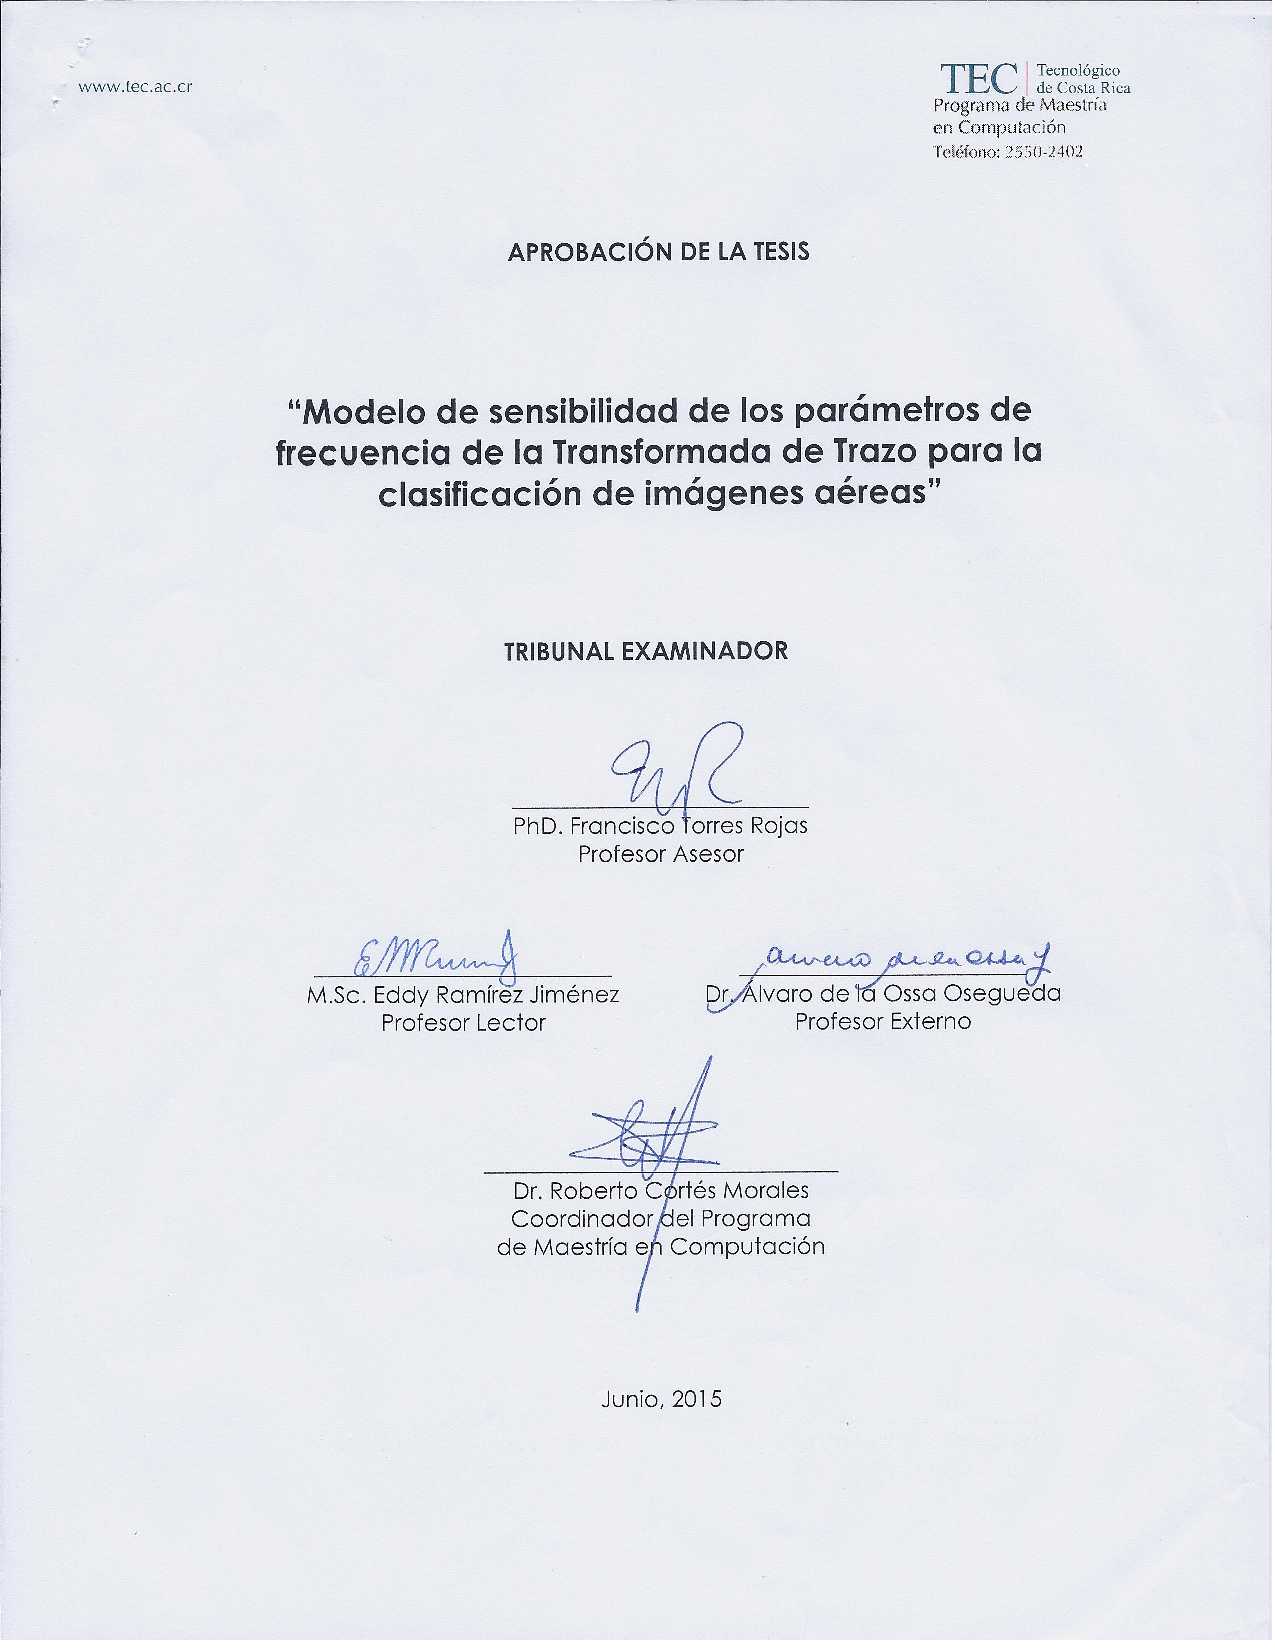
\includepdf[pages={1}]{body/aprobacion.pdf}


\chapter*{Agradecimientos}
\label{sect:Acknowledgment}

Quisiera agradecer a mis compañeros en el CNCA/CeNAT por su ayuda y consejo, en especial a Renato Garita y Álvaro de la Ossa.

A mi padre y madre por su compañía a lo largo de los años y no solo de esta investigación.

A mi tutor Francisco Torres por la oportunidad y la guía; a Andrés Messeguer y a Rodolfo Mora por su ayuda en las correcciones.

Al personal de la USES en la UCR, particularmente a María Isabel González, que sin su ayuda aún estaríamos buscando salidas.

\rule{0.5\textwidth}{0.5pt}\\

También agradecer al programa de becas CeNAT, que contribuyó a financiar parte de esta investigación.


\tableofcontents
\listoftables
\listoffigures
% Table of Symbols and Nomenclature
%\printnomenclature

\chapter{Acrónimos}

% Please keep it sorted by alphabetical order
\begin{acronym}

\acro{TT}{Transformada de trazo (siglas en inglés)}
\acro{TF}{Característica Triple (siglas en inglés)}
\acro{CeNAT}{Centro Nacional de Alta Tecnología} 
\acro{CNCA}{Colaboratorio Nacional de Computación Avanzada}
\acro{PRIAS}{Programa de Investigaciones Aerotransportadas y Sensores Remotos}
\acro{SVM}{Máquina de Soporte Vectorial (siglas en inglés)}
\acro{SMO}{Optimización Secuencial Mínima (siglas en inglés)}
\acro{Q-Q}{Cuantiles contra cuantiles}
\acro{RvVA}{Residuos contra Valores Ajustados}
\acro{ANOVA}{Análisis de varianza}


\end{acronym}

\mainmatter
% Use double space
\doublespacing
% Now fancy style
\pagestyle{fancy}
% Left the right header clean
\rhead{}


\chapter{Introducción y antecedentes}



\section{Introducción}
%Descripcion de la TT, y su historia%
%motivacion:
%claisificacion de imagenes aereas: generar mapas de cobertura automaticamente, facilitar el trabajo de los geografos, poder %realizar mapas de cobertura o clasificacion en campo. 

Actualmente en el Programa de Investigaciones Aerotransportadas y Sensores Remotos (PRIAS), uno de los laboratorios del Centro Nacional de Alta Tecnología (CeNAT) se crean mapas de cobertura de terreno utilizando imágenes aéreas o satelitales\cite{Biomarcc2013}. 

Los mapas de cobertura de terreno son una herramienta importante para los tomadores de decisiones, políticos, administrativos o directores en áreas como control de riesgo, gestión de desastres naturales o biodiversidad \cite{Biomarcc2013}, entre otros. Estos productos muestran de forma gráfica la distribución de algún atributo sobre un mapa \cite{Maps2014}.

Para construir dichos mapas se realiza un proceso en el cual el geógrafo toma la imagen y sobre ella marca polígonos según el tipo de terreno que sea. Este es un trabajo monótono y extenso, que se ha automatizado parcialmente con dos familias de métodos, los supervisados y los no-supervisados\cite{Chuvieco2010}. El PRIAS cuenta con alrededor de 13000 imágenes aéreas o satelitales sin procesar, provenientes de varios proyectos \cite{CARTA} \cite{RapidEye2012}.

El método de la Transformada de Trazo (TT), que dentro de los métodos automatizados cabe en los supervisados, \cite{Kadyrov2001} ha podido clasificar con éxito diferentes tipos de imágenes \cite{Bok2008} \cite{Srisuky2003} \cite{Petrou2007}. Este método extrae características asociadas a la imagen utilizando diferentes funcionales, uno tras el otro, para lograr una reducción en la dimensionalidad. Esta versión reducida de la imagen se conoce como característica triple (\emph{Triple Feature} o TF, por sus siglas en inglés) y es utilizada para la clasificación.

El Colaboratorio Nacional de Computación Avanzada (CNCA), también en el CeNAT, ha creado un prototipo de la TT y se han hecho pruebas de clasificación con datos experimentales y se esta preparando para hacer clasificaciones con datos reales \cite{Garita2013}.

%%es necesario utilizar varios funcinales y los mapas de ...
La TT puede tener un tiempo de ejecución considerable, dependiendo de varios factores que se explicaran más adelante. Con imágenes de 5000 $\times$ 5000 píxeles se ha tomado en promedio 3,7 horas \cite{Garita2013}. Para lograr una buena clasificación es necesario emplear varios funcionales y los mapas de cobertura utilizan imágenes de más de 4000 $\times$ 4000 píxeles \cite{RapidEye2012}. 

Debido a esto es necesario que la TT utilice parámetros que le permitan realizar su trabajo de forma eficiente. En esta tesis se explora el comportamiento de estos parámetros sobre imágenes aéreas. 

En el resto del capítulo 1, se detalla el funcionamiento de la TT y su complejidad computacional, el planteamiento del problema, la hipótesis de investigación y una revisión bibliográfica del trabajo relacionado.
En el capítulo 2 se enumeran los objetivos, general y específicos de la investigación, así como los alcances y limitaciones.
En el capítulo 3 se explican los dos experimentos que se desarrollaron para el estudio.
En el capítulo 4, se encuentran los resultados y el análisis de los mismos.
Por ultimo las conclusiones y el trabajo futuro aparecen en el capítulo 5.


\section{Transformada de trazo}
%Descripcion detallada del funcionamiento del algoritmo y sus caracteristicas de complejidad%
La TT es un método de extracción de características para su posterior clasificación. Este método se basa en trazar líneas sobre la imagen, de dónde se tomaran datos para ir transformándola a una versión más sencilla pero con igual poder de representación.

Una descripción detallada del algoritmo de extracción de características puede verse en \cite{Tutorial2008}, mas aquí se mencionarán los pasos más relevantes.

Es posible recorrer toda una imagen $I$ si se trazan líneas sobre toda la superficie de la imagen.
Estas líneas se definen con 2 parámetros: $\rho$ y $\phi$. Sea $o$ el centro de $I$. A partir de $o$ se define una distancia $\rho$ y un ángulo $\phi$. Se traza entonces una recta $\tau$, tangente al circulo de radio $\rho$ en el ángulo $\phi$, como se muestran en la figura \ref{fig:trazos}.

\begin{figure}[h!]
    \centering
    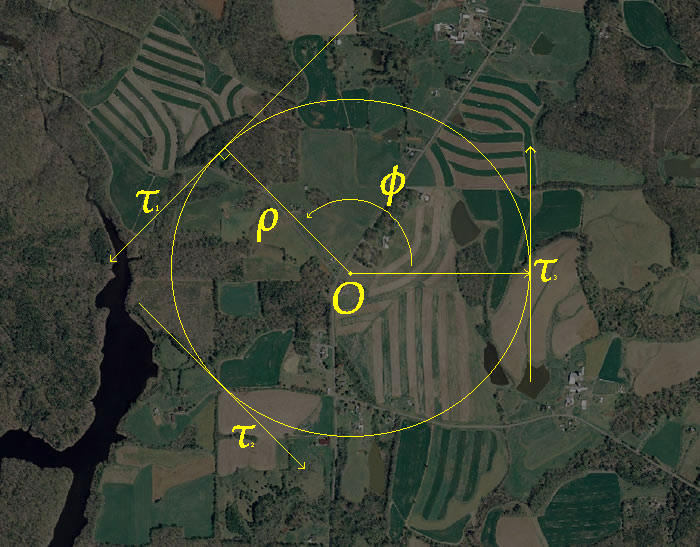
\includegraphics[width=1\textwidth]{images/trazos.png}
    \caption{Parametros de la TT. En la figura se presenta desde el punto de origen $O$, la rotación $\phi$, la distancia desde el origen $\rho$ y el trazo $\tau$ tangente al circulo de radio $\rho$.}
    \label{fig:trazos}
\end{figure}

El modelo también cuenta con 3 parámetros de frecuencia:
\begin{itemize}
    \item $\Delta \rho$: define cada cuántos píxeles se traza una línea. Si $\Delta \rho$ tiene un valor de 1 píxel se trazarán líneas cada píxel de la imagen, con un valor de 2 píxeles, cada 2 píxeles y así sucesivamente.
    \item $\Delta \phi$: determina cada cuántos grados se trazará una línea. Con un $\Delta \phi$ de 1º se trazarán líneas cada grado para un total de 360, con un valor de 90º, cada ángulo recto para un total de 4 líneas.
    \item $\Delta \tau$: fija, sobre la linea $\tau$, cuales píxeles se tomarán en cuenta para el procesamiento. Si $\Delta \tau$ se carga con un valor de 1 píxel, se utilizarán todos los píxeles de la línea, si tiene un valor de 2 píxeles se tomará una muestra cada 2 y así sucesivamente.
\end{itemize}

%%No es buena idea usar etc. 
Los píxeles que son intersecados por estas líneas $\tau$ y que cumplan con el parámetro $\Delta \tau$ serán la entrada para generar la primera representación de $I$, aplicando el funcional T o de trazo. El resultado será un arreglo de dos dimensiones (que puede ser interpretado como una imagen 2D), $I_T$, definida en parámetros de $\phi$ y $\rho$. El siguiente paso es tomar cada columna de $I_t$ y usarlas como entrada para el funcional P o diamétrico. Esto va a generar un arreglo $I_P$, que es una función del parámetro $\phi$. A este arreglo se le aplica el funcional $\Phi$ o de circo, para dar como resultado un sólo número $I_\Phi$ o característica triple. Este proceso se puede ver gráficamente en al figura \ref{fig:TT}.

Ahora bien, se da el caso en que no sólo es un funcional T, sino una serie, que se pueden indizar en una tabla de funcionales T. Esto produciría múltiples $I_T$ que se pueden denominar $I_T^\tau$, donde $\tau$ es el índice del funcional en la tabla de funcionales T. Esto puede ocurrir y es deseable que ocurra con las otras dos funcionales, ya que esto permite la creación de vectores de TF que puede ser más representativos de $I$ que una sola TF.

\begin{figure}[h!]
    \centering
    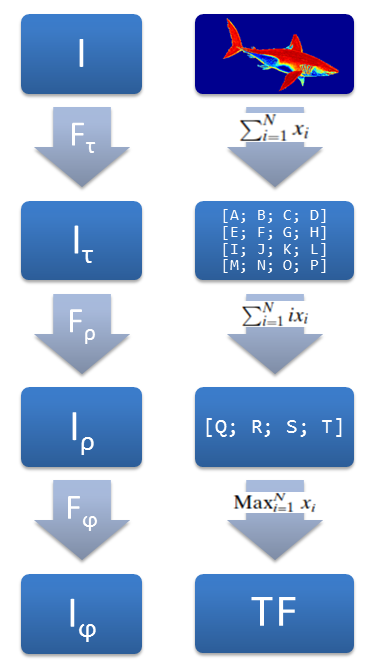
\includegraphics[width=0.5\textwidth]{images/tt.png}
    \caption{Representación gráfica del proceso de la Transformada de Trazo.}
    \label{fig:TT}
\end{figure}

%\bigskip\bigskip
Una vez obtenidas las TF para las imágenes originales, estos vectores de TF deben ser clasificados. Para esto es posible utilizar cualquier clasificador computacional, ya que al obtener una representación vectorial de la imagen se independiza del dominio original.
Clasificadores como redes neuronales artificiales, máquinas de soporte vectorial, agrupaciones, regresiones, entre otros, son todas técnicas válidas para realizar este paso\cite{Ethem2010}.
Como con cualquier clasificador, es necesario hacer una partición del conjunto original de datos; un subconjunto para el entrenamiento y otro para la clasificación.

\subsection{Complejidad de la Transformada de Trazo}

\begin{figure}[H]
    \begin{equation*}
        TF_{N_{\phi} N_{\rho} N_{\tau}} =
        \frac{C_{T}N_{T}n_{\tau}n_{\rho}n_{\phi}}{2} +
        C_{P}N_{P}N_{T}n_{\rho}n_{\phi} +
        C_{\phi}N_{\phi}N_{P}N_{T}n_{\phi}
    \end{equation*}
    \caption{Complejidad del algoritmo de la TT.}
    \label{eq:complejidad}
\end{figure}

La complejidad del algoritmo de la TT está dada por la ecuación de la figura \ref{eq:complejidad}, donde:
\begin{itemize}
    \item $TF_{N_{\phi} N_{\rho} N_{\tau}}$: Total de características triples generadas.
    \item $C_{T}$: cantidad de operaciones para la funcional de trazo hecha sobre cada muestra.
    \item $C_{P}$: cantidad de operaciones para la funcional diamétrica hecha por cada muestra.
    \item $C_{\phi}$: cantidad de operaciones para la funcional de circo hecha por cada muestra.
    \item $N_T$: cantidad de funcionales de trazo.
    \item $N_P$: cantidad de funcionales diamétricas.
    \item $N_\Phi$: cantidad de funcionales de circo.
    \item $n_\tau$: cantidad de muestras del parámetro $\tau$ a lo largo del trazo diagonal más extenso.
    \item $n_\rho$: cantidad de muestras del parámetro $\rho$.
    \item $n_{\phi}$: cantidad de muestras del parámetro $\phi$.
\end{itemize}

El primer término domina considerablemente la complejidad del algoritmo, dado que $n_\tau$, $n_\rho$ y $n_\phi$ son los términos que dependen del tamaño de la entrada mientras que $N_\tau$, $N_\rho$ y $N_\phi$ son los mismos para cualquier tamaño de entrada.

El parámetro de frecuencia $\Delta \tau$ está presente en los tres términos; está representado por $n_\tau$, por lo que es de especial importancia escoger un valor que minimice la cantidad de instrucciones. De igual forma ocurre con $\Delta \rho$ y $\Delta \phi$ pero en menor medida.


\section{Planteamiento del problema}
%Duracion es fea, no hay como saber q un valor para un parametro sea bueno o no, en articulos se han usado diferentes valores, pero no dicen xq. hacer el estudio

Como se mencionó previamente, la TT puede tener un tiempo de ejecución considerable, dependiendo de:
\begin{itemize}
    \item \textbf{Los funcionales utilizados}: existen 31 funcionales asociados a texturas \cite{Petrou2007} que han tenido éxito en sus procesos de clasificación. Son necesarias muchas características para lograr una buena clasificación \cite{Petrou2007}.
    \item \textbf{El tamaño de las imágenes}: las imágenes aéreas utilizadas en el PRIAS tienen tamaños de al menos 5000 $\times$ 5000 pixeles, lo cual es considerable si se toma en cuenta que los estudios anteriores trabajan sobre imágenes mucho más pequeñas \cite{Sayeed2001} \cite{Kadyrov2006} \cite{Albukhanajer2013} \cite{Srisuky2003} \cite{Petrou2007}.
    \item \textbf{Los parámetros de frecuencia (o $\Delta$)}: diferentes estudios muestran que variando estos parámetros es posible obtener buenos resultados \cite{Kadyrov2003} \cite{Petrou2007}, mas no existe un estudio que muestre como afectan estas frecuencias de muestreo a los resultados.
\end{itemize}

Si bien los dos primeros ítemes no se pueden cambiar, el tercero sí. Al no conocerse con exactitud el efecto que pueda tener las variaciones en los parámetros $\delta$ sobre la precisión y el tiempo de ejecución de la TT, se puede estar cayendo en alguna de estas dos situaciones: más trabajo del necesario para lograr una buena clasificación, o bien, es posible que con un poco más de trabajo se pueda lograr una clasificación con una tasa de precisión muy alta.

\section{Hipótesis}

%La Transformada de Trazo puede presentar mejores resultados estadísticamente, tanto en la precisión de la clasificación y/o en el tiempo de respuesta, variando los parámetros de frecuencia.
Basado en la ecuación de complejidad y la revisión del trabajo relacionado, se intuye que los parámetros de frecuencia pueden influir en el tiempo de extracción así como en la calidad de las TF que se generan para la clasificación, lo que lleva a plantear la siguiente hipótesis de investigación:\\

\begin{large}
\textit{La Transformada de Trazo presenta mejores resultados estadísticamente, en precisión de clasificación y en tiempo de extracción de características, al variar los parámetros de frecuencia, el tipo de clasificador y el tipo de cobertura.}
\end{large}

  
\section{Trabajo relacionado}
% articulos donde se ha planeatedo uso distinto de los parametros

Desde la elaboración conceptual de la TT en el 2001 \cite{Kadyrov2001}, esta ha producido varias publicaciones de casos de estudio en diferentes áreas.
%% uso historico o previo

La TT es una generalización de la transformada de Radon \cite{Ginkel2004} \cite{Kadyrov2003} en la que se calcula como funcional de trazo la integral del mismo trazo. Este método ha sido utilizado en tomografía e imagenología médica \cite{Tutorial2008}.

Previo a la publicación de la TT, ya se manejaba la idea de extraer características invariantes de imágenes para la clasificación. En \cite{Sayeed2001}, se realizó una extracción de características para determinar si un paciente padecía de Alzheimer. Dicho estudio tuvo una precisión del 88\% al clasificar dichas imágenes.
%% exitos en clasificacion


Es posible identificar huellas de insectos utilizando la TT junto con otros métodos para la segmentación de imágenes. En \cite{Bok2008} se muestra una mejora de entre 7\% y 63\% en comparación con el método convencional \cite{Shin2007}.

La TT se puede combinar con otros métodos para extraer características robustas. La combinación con algoritmos evolutivos mostró que da buenos resultados al clasificar TF \cite{Albukhanajer2013}.

Las características de invarianza o sensibilidad de las TF se pueden comparar en \cite{Turan2005}. Aquí una serie de imágenes de referencia se compara con imágenes que han sido sujetas a transformaciones afines: rotación, desplazamiento y escalamiento. El estudio concluyó que la TT, usando la combinación de funcionales correctas tiene una precisión de entre 98\% y 100\%.

La TT se puede utilizar para clasificar o reconocer imágenes más complejas como rostros. En \cite{Srisuky2003} se compara el método Eigenfaces\cite{Zhang1997} con una modificación de la TT llamada: ``Masked Trace Transform'' + ``Weighted Trace Transform''. El método basado en la TT tuvo mejor desempeño en modificaciones como rotación, escalamiento y cambio en la expresión facial.
%% exitos en clasificacion con texturas

%% uso de distintos deltas
La variación de parámetros para producir las TF no es muy común y se utiliza una configuración estándar. Aun así, hay varios estudios donde se obtuvieron buenos resultados. En \cite{Kadyrov2003} se realizaron experimentos para crear firmas únicas para imágenes utilizando características extraídas con la TT. Aquí, los parámetros para $\Delta \rho$, $\Delta \tau$ y $\Delta \phi$ fueron respectivamente, 2 píxeles, 2 píxeles  y 3º. El estudio reveló que las TF tienen un desempeño similar a las características extraídas con otros métodos, pero las primeras son más robustas y resistentes al cambio.

En \cite{Petrou2007} se comparan las características extraídas por métodos automáticos como la TT contra otros más rígidos como con el uso de matrices de co-ocurrencia, con base a la forma en como las personas interpretan las texturas. En general, las características extraídas con la TT se puede modelar de manera semejante a la forma en que los humanos perciben las texturas. En los experimentos realizados en este estudio, se utilizó, a diferencia de los experimentos previos, un $\Delta \rho$ de 2.





\chapter{Objetivos y aportes}

\section{Objetivo general}

Estudiar el comportamiento de la TT en términos de precisión y tiempo de extracción de características, utilizando diferentes modelos de parámetros, clasificadores y tipos de terreno.

\section{Objetivos específicos}

\begin{enumerate}
    \item Comparar el tiempo de extracción de características y precisión de la clasificación de la TT utilizando diferentes combinaciones de los parámetros de frecuencia, cuatro distintos clasificadores y cinco tipos de cobertura de terreno.
    \item Analizar estadísticamente los resultados observados para determinar la influencia de los parámetros en el tiempo de extracción de características y precisión de la clasificación
\end{enumerate}
    
    
\section{Alcances y limitaciones}

Dentro del alcance de esta propuesta se definen los siguientes entregables:
\begin{enumerate}
    \item Prototipo de un programa para la extracción de características usando la TT. En este prototipo deben ser parametrizables, los parámetros de frecuencia y el clasificador.
    \item Prototipo de los clasificadores.
    \item Programas auxiliares para la ejecución y el control de los dos anteriores.
    \item Análisis estadístico para contrastar los resultados de los experimentos.
    \item Artículo científico que se entregará al comité editorial de alguna revista o conferencia, con miras a su publicación.
\end{enumerate}

Por motivos de tiempo y extensión, en esta investigación no se tomarán en cuenta:
\begin{itemize}
    \item Imágenes con formas irregulares, sólo se utilizarán imágenes rectangulares.
    \item Imágenes de tamaños variables. Se utilizarán imágenes en formato PNG, con un tamaño de $500 \times 500$ píxeles.
    \item Funcionales fuera de aquellas revisadas en la literatura. Se utilizarán los funcionales descritas en \cite{Petrou2007}.
    \item Una ventana de análisis en la imagen, ni deslizante ni de tamaño variable. La ventana de análisis será del tamaño total de la imagen.
\end{itemize}

Tampoco es la intención de esta investigación presentar un sistema completo para la clasificación de imágenes o para la generación de mapas de cobertura.

Por último, no se tomará en cuenta cualquier otro resultado, documento, software o producción que no esté contemplado en esta propuesta.

\chapter{Experimentación} 

Con el fin de dar evidencia a favor de la hipótesis, se diseñaron dos experimentos siguiendo la metodología del diseño multifactorial\cite{Montgomery2001}.
%En estos, la idea es medir la sensibilidad de las respuestas: tiempo de extracción y precisión de la clasificación cuando los parámetros de frecuencia se alejan de la configuración original de $\Delta \tau$=1, $\Delta \rho$=1 $\Delta \phi$=1º.

Los resultados de ambos experimentos se estudiaran por medio de un \textbf{Análisis de Varianza}\cite{Montgomery2001} (ANOVA por sus siglas en inglés). Aquí se toman $n$ muestras de $k$ poblaciones y estos datos se estudian para confirmar que vienen de un mismo origen (o sea, que todos se comportan estadísticamente igual) o no.

Es necesario establecer una hipótesis nula y una alternativa:
\begin{itemize}
    \item Hipótesis nula $H_0$: la media entre los grupos estudiados es la misma y no afecta el resultado.
    
    $\mu_0 = \mu_1 = ... = \mu_n$.
    \item Hipótesis alternativa $H_1$: la media de al menos uno de los grupos estudiados es diferente y afecta el resultado.
    
    $\exists i,j / \mu_i \neq \mu_j$.
\end{itemize}


\section{Experimento A: Tiempo de ejecución de la extracción de características}

El primer experimento se realizó para medir la influencia de los parámetros de frecuencia y del tipo de cobertura de terreno sobre la variable de respuesta, el \textbf{tiempo requerido para generar las características} de una imagen. Siguiendo el modelo multifactorial\cite{Montgomery2001}, los niveles y factores para el experimento A fueron:
\begin{itemize}
    \item $\Delta \tau$ (píxeles): 1, 2 y 3.
    \item $\Delta \rho$ (píxeles): 1, 2 y 3.
    \item $\Delta \phi$ (grados): 0,5º, 1º y 2º.
    \item Cobertura de terreno (tipos): bosque, agua, rural, urbano y sembradío.
\end{itemize}

Con 32 imágenes por tipo de cobertura y los niveles de las variables anteriores, se tienen 4320 ($3\times3\times3\times32\times5$) ejecuciones por cada una de las tres réplicas. Esto suma un gran total de 12960 ejecuciones de la TT.

Por cada ejecución de la TT se producen dos resultados: un arreglo de TF por cada imagen y el tiempo de ejecución de la extracción de características. El primero se utilizó para el experimento B y el segundo se evaluó con ANOVA.

A continuación se explican los detalles del experimento A.

\subsection{Conjunto de imágenes}

Las imágenes utilizadas para la extracción de características provienen del proyecto Carta 2005\cite{CARTA} y fueron proporcionadas por el PRIAS. A su vez, éstas fueron recortadas y clasificadas previamente por un experto geógrafo. 

Se contó con 32 imágenes por tipo de cobertura, lo que suma 160 imágenes en total. Cada imagen tiene una dimensión de $500 \times 500$ píxeles almacenadas en formato PNG y se eligió este tamaño previendo el tiempo de extracción de alrededor 130 segundos por imagen, según \cite{Garita2013}.

El cuadro \ref{fig:types} muestra diferentes ejemplos de cada tipo de textura. En la primera fila se muestran texturas más homogéneas y en la segunda filas texturas más heterogéneas de cada tipo de cobertura.

%\begin{figure}[h]
%    \centering
    \begin{table}
    \setlength{\tabcolsep}{0.2pt}
    \renewcommand{\arraystretch}{0.1}
        \begin{tabular}{ ccccc }
            
            
            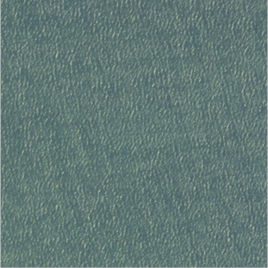
\includegraphics[width=0.2\textwidth]{images/tipos/Au.png}& 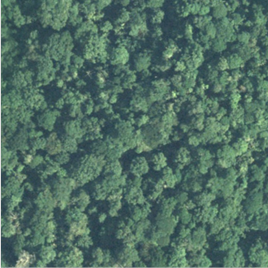
\includegraphics[width=0.2\textwidth]{images/tipos/Bu.png}& 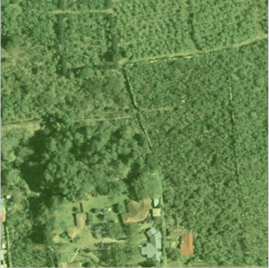
\includegraphics[width=0.2\textwidth]{images/tipos/Ru.png}& 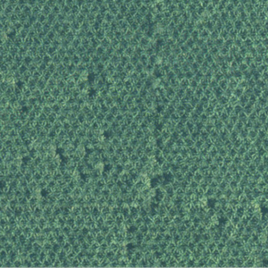
\includegraphics[width=0.2\textwidth]{images/tipos/Pu.png}& 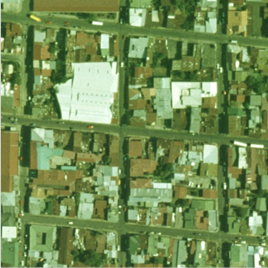
\includegraphics[width=0.2\textwidth]{images/tipos/Uu.png}\\
            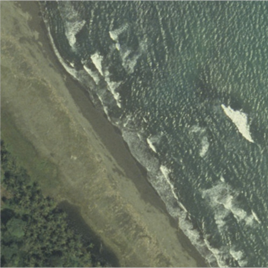
\includegraphics[width=0.2\textwidth]{images/tipos/Ad.png}& 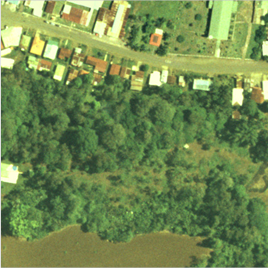
\includegraphics[width=0.2\textwidth]{images/tipos/Bd.png}& 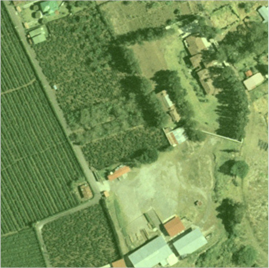
\includegraphics[width=0.2\textwidth]{images/tipos/Rd.png}& 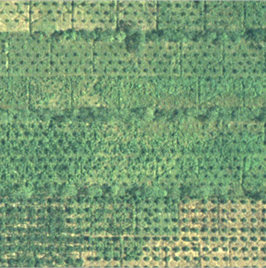
\includegraphics[width=0.2\textwidth]{images/tipos/Pd.png}& 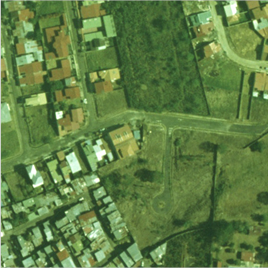
\includegraphics[width=0.2\textwidth]{images/tipos/Ud.png}\\
            &&&&\\
            &&&&\\
            &&&&\\
            Agua & Bosque & Rural & Sembradío & Urbano \\
            
        \end{tabular}
        \caption{Ejemplo de tipos de cobertura. Cada columna presenta dos imágenes de un tipo de cobertura distinto, respectivamente: agua, bosque, rural, sembradío y urbano.}
        \label{fig:types}
    \end{table}
    
    %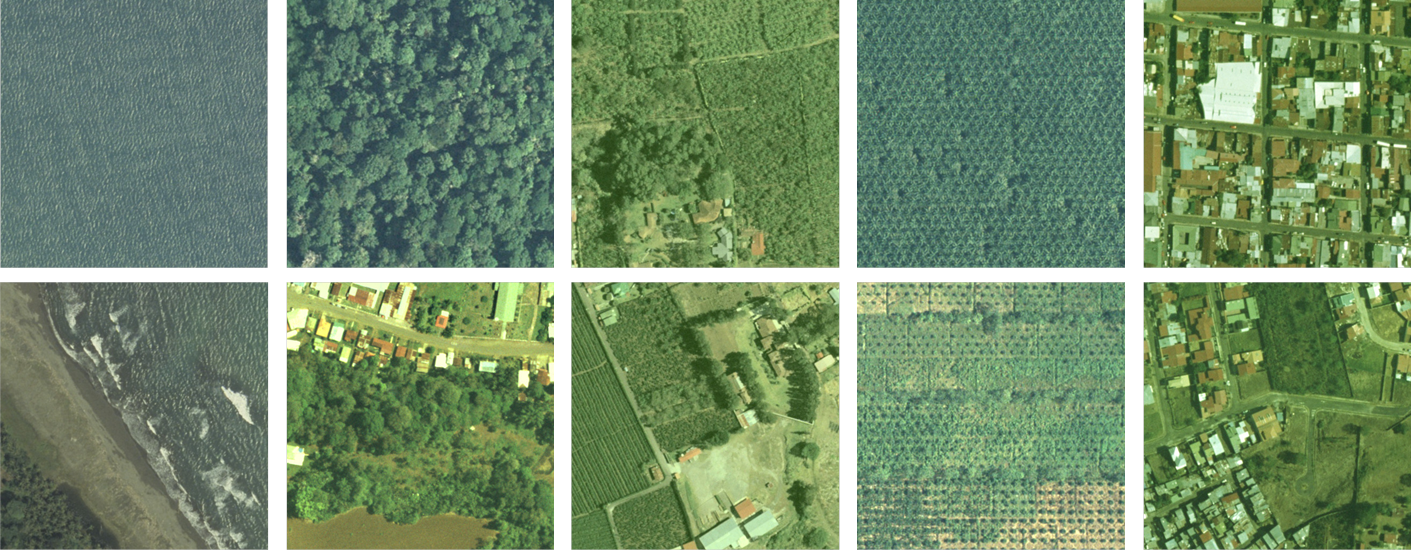
\includegraphics[width=1\textwidth]{images/tipos.png}
    
%\end{figure}


\subsection{Funcionales}

Las funcionales utilizadas en cada uno de los tres pasos de reducción son críticas para extraer características útiles para la etapa de clasificación y puede en realidad ser un tema de investigación por sí solo. Es por esto que las funcionales que se utilizaron en el experimento A son aquellas que mostraron buenos resultados al clasificar texturas en \cite{Petrou2007} y \cite{Tutorial2008}.\\

\begin{longtable}{ |c|l| }
        \hline 
        \textbf{\#} & \textbf{Funcional} \\
        \hline 
        \endhead
        
    	1.&$\sum \limits_{i=1}^{N}{x_i}$ \\ \hline
    	2.&$\sum \limits_{i=1}^{N}{ix_i}$\\ \hline
    	3.&$\frac{1}{N}\sqrt{\sum \limits_{i=1}^{N}{(x_i-\hat{x})^2}}$  \\ \hline
    	4.&$\sqrt{\sum \limits_{i=1}^{N}{x_i^2}}$  \\ \hline
    	5.&$\max \limits_{ i=1}^{N}{x_i}$  \\ \hline
    	6.&$\sum \limits_{i=1}^{N-1}{|{x_{i+1}-x_i}|}$  \\ \hline
    	7.&$\sum \limits_{i=1}^{N-1}{|{x_{i+1}-x_i}|}^2$  \\ \hline
    	8.&$\sum \limits_{i=4}^{N-3}{|{x_{i-3}+x_{i-2}+x_{i-1}-x_{i+1}-x_{i+2}-x_{i+3}}|}$  \\ \hline
    	9.&$\sum \limits_{i=3}^{N-2}{|{x_{i-2}+x_{i-1}-x_{i+1}-x_{i+2}}|}$  \\ \hline
    	10.&$\sum \limits_{i=5}^{N-4}{|{x_{i-4}+x_{i-3}+...+x_{i-1}-x_{i+1}-...-x_{i+3}-x_{i+4}}|}$  \\ \hline
    	11.&$\sum \limits_{i=6}^{N-5}{|{x_{i-5}+x_{i-4}+...+x_{i-1}-x_{i+1}-...-x_{i+4}-x_{i+5}}|}$  \\ \hline
    	12.&$\sum \limits_{i=7}^{N-6}{|{x_{i-6}+x_{i-5}+...+x_{i-1}-x_{i+1}-...-x_{i+5}-x_{i+6}}|}$  \\ \hline
    	13.&$\sum \limits_{i=8}^{N-7}{|{x_{i-7}+x_{i-6}+...+x_{i-1}-x_{i+1}-...-x_{i+6}-x_{i+7}}|}$  \\ \hline
    	14.&$\sum \limits_{i=5}^{N-4}\sum \limits_{k=1}^{4}{|{x_{i-k}-x_{i+k}}|}$  \\ \hline
    	15.&$\sum \limits_{i=6}^{N-5}\sum \limits_{k=1}^{5}{|{x_{i-k}-x_{i+k}}|}$  \\ \hline
    	16.&$\sum \limits_{i=7}^{N-6}\sum \limits_{k=1}^{6}{|{x_{i-k}-x_{i+k}}|}$  \\ \hline
    	17.&$\sum \limits_{i=8}^{N-7}\sum \limits_{k=1}^{7}{|{x_{i-k}-x_{i+k}}|}$  \\ \hline
    	18.&$\sum \limits_{i=11}^{N-10}\sum \limits_{k=1}^{10}{|{x_{i-k}-x_{i+k}}|}$  \\ \hline
    	19.&$\sum \limits_{i=16}^{N-15}\sum \limits_{k=1}^{15}{|{x_{i-k}-x_{i+k}}|}$  \\ \hline
    	20.&$\sum \limits_{i=21}^{N-20}\sum \limits_{k=1}^{20}{|{x_{i-k}-x_{i+k}}|}$  \\ \hline
    	21.&$\sum \limits_{i=26}^{N-25}\sum \limits_{k=1}^{25}{|{x_{i-k}-x_{i+k}}|}$  \\ \hline
    	22.&$\sum \limits_{i=11}^{N-10}((1+\sum \limits_{k=1}^{10}{|{x_{i-k}-x_{i+k}})/(1+\sum \limits_{k=-10}^{9}{|{x_{i-k}-x_{i+k}}|}}))$  \\ \hline
    	23.&$\sum \limits \limits_{i=11}^{N-10}\sqrt{|(\sum \limits_{k=1}^{10}{|{x_{i-k}-x_{i+k}})^2/(1+\sum \limits_{k=-10}^{9}{|{x_{i-k}-x_{i+k}}|}})|}$  \\ \hline
    	24.&$\sum \limits_{i=1}^{N-2}{|{x_{i}-2x_{i+1}+x_{i+2}}|}$  \\ \hline
    	25.&$\sum \limits_{i=1}^{N-3}{|{x_{i}-3x_{i+1}+3x_{i+2}-x_{i+3}}|}$  \\ \hline
    	26.&$\sum \limits_{i=1}^{N-4}{|{x_{i}-4x_{i+1}+6x_{i+2}-4x_{i+3}+x_{i+4}}|}$  \\ \hline
    	27.&$\sum \limits_{i=1}^{N-5}{|{x_{i}-5x_{i+1}+10x_{i+2}-10x_{i+3}+5x_{i+4}-x_{i+4}}|}$  \\ \hline
    	28.&$\sum \limits_{i=1}^{N-2}{|{x_{i}-2x_{i+1}+x_{i+2}}x_{i+1}|}$  \\ \hline
    	29.&$\sum \limits_{i=1}^{N-3}{|{x_{i}-3x_{i+1}+3x_{i+2}-x_{i+3}}x_{i+1}|}$  \\ \hline
    	30.&$\sum \limits_{i=1}^{N-4}{|{x_{i}-4x_{i+1}+6x_{i+2}-4x_{i+3}+x_{i+4}}x_{i+2}|}$  \\ \hline
    	31.&$\sum \limits_{i=1}^{N-5}{|{x_{i}-5x_{i+1}+10x_{i+2}-10x_{i+3}+5x_{i+4}-x_{i+4}}x_{i+2}|}$ \\ \hline
    \caption{Funcionales de trazo utilizadas en la extracción de características.}
    \label{tab:ft}
\end{longtable}


%Las 31 funcionales de trazo utilizadas fueron:
%\begin{enumerate}
%\item $\sum \limits_{i=1}^{N}{x_i}$ 
%\item $\sum \limits_{i=1}^{N}{ix_i}$
%\item $\frac{1}{N}\sqrt{\sum \limits_{i=1}^{N}{(x_i-\hat{x})^2}}$  
%\item $\sqrt{\sum \limits_{i=1}^{N}{x_i^2}}$  
%\item $\max \limits_{ i=1}^{N}{x_i}$  
%\item $\sum \limits_{i=1}^{N-1}{|{x_{i+1}-x_i}|}$  
%\item $\sum \limits_{i=1}^{N-1}{|{x_{i+1}-x_i}|}^2$  
%\item $\sum \limits_{i=4}^{N-3}{|{x_{i-3}+x_{i-2}+x_{i-1}-x_{i+1}-x_{i+2}-x_{i+3}}|}$  
%\item $\sum \limits_{i=3}^{N-2}{|{x_{i-2}+x_{i-1}-x_{i+1}-x_{i+2}}|}$  
%\item $\sum \limits_{i=5}^{N-4}{|{x_{i-4}+x_{i-3}+...+x_{i-1}-x_{i+1}-...-x_{i+3}-x_{i+4}}|}$  
%\item $\sum \limits_{i=6}^{N-5}{|{x_{i-5}+x_{i-4}+...+x_{i-1}-x_{i+1}-...-x_{i+4}-x_{i+5}}|}$  
%\item $\sum \limits_{i=7}^{N-6}{|{x_{i-6}+x_{i-5}+...+x_{i-1}-x_{i+1}-...-x_{i+5}-x_{i+6}}|}$  
%\item $\sum \limits_{i=8}^{N-7}{|{x_{i-7}+x_{i-6}+...+x_{i-1}-x_{i+1}-...-x_{i+6}-x_{i+7}}|}$  
%\item $\sum \limits_{i=5}^{N-4}\sum \limits_{k=1}^{4}{|{x_{i-k}-x_{i+k}}|}$  
%\item $\sum \limits_{i=6}^{N-5}\sum \limits_{k=1}^{5}{|{x_{i-k}-x_{i+k}}|}$  
%\item $\sum \limits_{i=7}^{N-6}\sum \limits_{k=1}^{6}{|{x_{i-k}-x_{i+k}}|}$  
%\item $\sum \limits_{i=8}^{N-7}\sum \limits_{k=1}^{7}{|{x_{i-k}-x_{i+k}}|}$  
%\item $\sum \limits_{i=11}^{N-10}\sum \limits_{k=1}^{10}{|{x_{i-k}-x_{i+k}}|}$  
%\item $\sum \limits_{i=16}^{N-15}\sum \limits_{k=1}^{15}{|{x_{i-k}-x_{i+k}}|}$  
%\item $\sum \limits_{i=21}^{N-20}\sum \limits_{k=1}^{20}{|{x_{i-k}-x_{i+k}}|}$  
%\item $\sum \limits_{i=26}^{N-25}\sum \limits_{k=1}^{25}{|{x_{i-k}-x_{i+k}}|}$  
%\item $\sum \limits_{i=11}^{N-10}((1+\sum \limits_{k=1}^{10}{|{x_{i-k}-x_{i+k}})/(1+\sum \limits_{k=-10}^{9}{|{x_{i-k}-x_{i+k}}|}}))$  
%\item $\sum \limits \limits_{i=11}^{N-10}\sqrt{|(\sum \limits_{k=1}^{10}{|{x_{i-k}-x_{i+k}})^2/(1+\sum \limits_{k=-10}^{9}{|{x_{i-k}-x_{i+k}}|}})|}$  
%\item $\sum \limits_{i=1}^{N-2}{|{x_{i}-2x_{i+1}+x_{i+2}}|}$  
%\item $\sum \limits_{i=1}^{N-3}{|{x_{i}-3x_{i+1}+3x_{i+2}-x_{i+3}}|}$  
%\item $\sum \limits_{i=1}^{N-4}{|{x_{i}-4x_{i+1}+6x_{i+2}-4x_{i+3}+x_{i+4}}|}$  
%\item $\sum \limits_{i=1}^{N-5}{|{x_{i}-5x_{i+1}+10x_{i+2}-10x_{i+3}+5x_{i+4}-x_{i+4}}|}$  
%\item $\sum \limits_{i=1}^{N-2}{|{x_{i}-2x_{i+1}+x_{i+2}}x_{i+1}|}$  
%\item $\sum \limits_{i=1}^{N-3}{|{x_{i}-3x_{i+1}+3x_{i+2}-x_{i+3}}x_{i+1}|}$  
%\item $\sum \limits_{i=1}^{N-4}{|{x_{i}-4x_{i+1}+6x_{i+2}-4x_{i+3}+x_{i+4}}x_{i+2}|}$  
%\item $\sum \limits_{i=1}^{N-5}{|{x_{i}-5x_{i+1}+10x_{i+2}-10x_{i+3}+5x_{i+4}-x_{i+4}}x_{i+2}|}$ 
%\end{enumerate}


Las 31 funcionales de trazo se presentan en el cuadro \ref{tab:ft}.
Muchas de las funcionales utilizadas aquí exploran un área sobre $\tau$. Por ejemplo, las funcionales 10, 11, 12 y 13 suman, dado el punto de tangencia, el valor de los píxeles en ambas direcciones de la recta; cada vez en un vecindario más grande. Otras funcionales calculan valores interesantes del trazo, el punto máximo (5) o la suma de todos los puntos (1).\\


\begin{longtable}{ |c|l| }
        \hline
        \textbf{\#} & \textbf{Funcional} \\
        \hline
        \endhead
1.&$\max \limits_{i=1}^{N}{x_i}$\\ \hline
2.&$\min \limits_{i=1}^{N}{x_i}$\\ \hline
3.&$\sqrt{\sum \limits_{i=1}^{N}{x_i^2}}$ \\ \hline
4.&$\frac{\sum \limits_{i=1}^{N}{ix_i}}{\sum \limits_{i=1}^{N}{x_i}}$ \\ \hline
5.&$\sum \limits_{i=1}^{N}{ix_i}$ \\ \hline
6.&$\frac{1}{N}\sum_{i=1}^{N}{(x_i-\hat{x})^2}$ \\ \hline
7.&$c$ tal que:$\sum \limits_{i=1}^{c}{x_i}=\sum \limits_{i=c}^{N}{x_i}$ \\ \hline
8.&$\sum \limits_{i=1}^{N-1}{|x_{i+1}-x_{i}|}$ \\ \hline
9.&$c$ tal que:$\sum \limits_{i=1}^{c}{|x_{i+1}-x_{i}|}=\sum \limits_{i=c}^{N-1}{|x_{i+1}-x_{i}|}$ \\ \hline
10.&$\sum \limits_{i=1}^{N-4}{|x_{i}-4x_{i+1}+6x_{i+2}-4x_{i+3}+x_{i+4}|}$ \\ \hline
    \caption{Funcionales diamétricas utilizadas en la extracción de características.}
    \label{tab:fd}
\end{longtable}

%\begin{enumerate}
%\item $\max \limits_{i=1}^{N}{x_i}$
%\item $\min \limits_{i=1}^{N}{x_i}$
%\item $\sqrt{\sum \limits_{i=1}^{N}{x_i^2}}$ 
%\item $\frac{\sum \limits_{i=1}^{N}{ix_i}}{\sum \limits_{i=1}^{N}{x_i}}$ 
%\item $\sum \limits_{i=1}^{N}{ix_i}$ 
%\item $\frac{1}{N}\sum_{i=1}^{N}{(x_i-\hat{x})^2}$ 
%\item $c$ tal que: $\sum \limits_{i=1}^{c}{x_i}=\sum \limits_{i=c}^{N}{x_i}$ 
%\item $\sum \limits_{i=1}^{N-1}{|x_{i+1}-x_{i}|}$ 
%\item $c$ tal que: $\sum \limits_{i=1}^{c}{|x_{i+1}-x_{i}|}=\sum \limits_{i=c}^{N-1}{|x_{i+1}-x_{i}|}$ 
%\item $\sum \limits_{i=1}^{N-4}{|x_{i}-4x_{i+1}+6x_{i+2}-4x_{i+3}+x_{i+4}|}$ 
%\end{enumerate}


Las 10 funcionales de diámetro utilizadas se presentan en el cuadro \ref{tab:fd}.
De estas, algunas son de la misma familia que varias funcionales de trazo, pero aparecen aquí algunas totalmente distintas, como la 7 y la 9. En la 7, se calcula un número $c$ sobre el trazo en donde la suma de los píxeles antes de $c$ sea igual a la suma de los píxeles luego de $c$, esto con el fin de encontrar un punto de equilibrio sobre el trazo. En caso de no existir, se utiliza el valor de 0.\\

%Las 18 funcionales de circo utilizadas fueron:
%\begin{enumerate}
%\item $\sum \limits_{i=1}^{N-1}{|x_{i+1}-x_{i}|^2}$
%\item $\sum \limits_{i=1}^{N-1}{|x_{i+1}-x_{i}|}$
%\item $\sqrt{\sum \limits_{i=1}^{N}{x_i^2}}$ 
%\item $\sum \limits_{i=1}^{N}{x_i}$ 
%\item $\max \limits_{i=1}^{N}{x_i}$ 
%\item $\max \limits_{i=1}^{N}{x_i}-\min \limits_{i=1}^{N}{x_i}$ 
%\item $i$ tal que $x_i=\min \limits_{i=1}^{N}{x_i}$ 
%\item $i$ tal que $x_i=\max \limits_{i=1}^{N}{x_i}$ 
%\item $i$ tal que $x_i=\min \limits_{i=1}^{N}{x_i}$ sin la primera armónica 
%\item $i$ tal que $x_i=\max \limits_{i=1}^{N}{x_i}$ sin la primera armónica 
%\item Amplitud de la primera armónica 
%\item Fase de la primera armónica 
%\item Amplitud de la segunda armónica 
%\item Fase de la segunda armónica 
%\item Amplitud de la tercera armónica 
%\item Fase de la tercera armónica 
%\item Amplitud de la cuarta armónica 
%\item Fase de la cuarta armónica 
%\end{enumerate}


\begin{longtable}{ |c|l| }
        
        \hline
        \textbf{\#} & \textbf{Funcional} \\
        \hline
        \endhead
        
        1.&$\sum \limits_{i=1}^{N-1}{|x_{i+1}-x_{i}|^2}$\\ \hline
    2.&$\sum \limits_{i=1}^{N-1}{|x_{i+1}-x_{i}|}$\\ \hline
    3.&$\sqrt{\sum \limits_{i=1}^{N}{x_i^2}}$ \\ \hline
    4.&$\sum \limits_{i=1}^{N}{x_i}$ \\ \hline
    5.&$\max \limits_{i=1}^{N}{x_i}$ \\ \hline
    6.&$\max \limits_{i=1}^{N}{x_i}-\min \limits_{i=1}^{N}{x_i}$ \\ \hline
    7.&$i$ tal que $x_i=\min \limits_{i=1}^{N}{x_i}$ \\ \hline
    8.&$i$ tal que $x_i=\max \limits_{i=1}^{N}{x_i}$ \\ \hline
    9.&$i$ tal que $x_i=\min \limits_{i=1}^{N}{x_i}$ sin la primera armónica \\ \hline
    10.&$i$ tal que $x_i=\max \limits_{i=1}^{N}{x_i}$ sin la primera armónica \\ \hline
    11.&Amplitud de la primera armónica \\ \hline
    12.&Fase de la primera armónica \\ \hline
    13.&Amplitud de la segunda armónica \\ \hline
    14.&Fase de la segunda armónica \\ \hline
    15.&Amplitud de la tercera armónica \\ \hline
    16.&Fase de la tercera armónica \\ \hline
    17.&Amplitud de la cuarta armónica \\ \hline
    18.&Fase de la cuarta armónica \\ \hline
    
            
    \caption{Funcionales de circo utilizadas en la extracción de características.}
    \label{tab:fc}
\end{longtable}

Las funcionales de circo se presentan en el cuardo \ref{tab:fc} e introducen propiedades de las armónicas de las transformadas diamétricas interpretadas como ondas (de la 11 a la 18). Éstas exponen características físicas que puede facilitar la identificación de las imágenes originales.

\subsection{Implementación del algoritmo de la TT}

La implementación de la TT se basó en el código \cite{Garita2014}. Esta consiste de 3 etapas: 

\begin{enumerate}
    
    \item \textbf{Carga de imágenes}
    %%%%%%%%%%%%%%%%%%%%%%%%%%
    
    Las imágenes se cargan una a la vez, y en el caso de tener que procesar múltiples imágenes se puede utilizar paralelismo a nivel de tareas (programas) y cargar una imagen por cada programa.
    La carga de imágenes se realizó utilizando la biblioteca para manipulación de imágenes \textit{ImageMagick}\footnote{http://www.imagemagick.org/}. Es necesario convertir los píxeles de la imagen a una representación en escala de grises, lo cual se lleva a cabo con la función \texttt{MagickQuantizeImage} \cite{ImageMagick2015}, usando como tercer parámetro \texttt{GRAYColorspace}. Esta función analiza los colores de la imagen y los mapea al espacio lineal de grises usando el algoritmo \texttt{quantize}\cite{quantize2015}. Esto permite utilizar una sola capa de color para el cálculo de las funcionales. Una vez que se haya levantado la imagen en memoria, se pasa a la segunda etapa de preprocesamiento.
    
    
    \item \textbf{Preprocesamiento de las imágenes}
    %%%%%%%%%%%%%%%%%%%%%%%%%%
    
    La etapa de preprocesamiento calcula datos comunes que serán utilizados durante la extracción de características con el fin de no tener que recomputarlos. Aquí es importante tomar en cuenta las características de memoria del equipo donde corre la implementación, ya que por cada imagen se debe almacenar una cantidad considerable de información que tiene una relación directa con el tamaño de la imagen y los parámetros $\Delta$. Estos son:
    \begin{itemize}
        \item Alto y Ancho.
        \item $\Delta \tau$, $\Delta \rho$ y $\Delta \phi$.
        \item Tamaño de la cuadrícula, dependiente de la arquitectura para máximizar el detalle.
        \item Píxel de inicio y fin de cada trazo.
        \item El desplazamiento en los ejes $x$ y $y$ para cada trazo, dependiente de los parámetros $\Delta$.
    \end{itemize}
    
    
    \item  \textbf{Extracción de características}
    %%%%%%%%%%%%%%%%%%%%%%%%%%
    
    Por último, se aplican los tres juegos de funcionales a los datos. Primero, se seleccionan los puntos involucrados en las funcionales de trazo, utilizando los datos precalculados en la etapa anterior, para luego aplicar de forma iterativa todas las funcionales.
    Cada funcional de cada paso (trazo, diamétrica o de circo) podría ser ejecutada de forma independiente ya que la dependencia existe entre cada juego de funcionales y no entre las funcionales de cada juego. El pseudocódigo en el algoritmo \ref{fig:extraccion} muestra este proceso.\\
    
    \begin{algorithm}[h]
    \floatname{algorithm}{Algoritmo}
        \begin{algorithmic}
            \State $I =$ Imagen a procesar
            
            \For{$a$ en ángulos a procesar} 
            
                \For{$d$ en trazos a procesar} 
                    
                    \For{$t$ en puntos a procesar} 
                        \LineComment{Calcular las funcionales de trazo}
                        \State $I_{\tau} = $ calcularFuncionalesTrazo($I$, $a$, $d$, $t$)
                    \EndFor
                \EndFor
    
                \LineComment{Luego de procesadas todas las funcionales de trazo}
                \For{$d$ en trazos a procesar} 
                    \LineComment{Calcular las funcionales diamétricas para cada funcional de trazo}
                    \State $I_{\rho} = $ calcularFuncionalesDiametrica($I_{\tau}$)
                \EndFor
            
            \EndFor
            \LineComment{Luego de procesadas todas las funcionales de trazo y diamétricas}
            
            \For{$a$ en ángulos a procesar} 
                \LineComment{Calcular las funcionales de circo para cada funcional trazo+diamétrica}
                \State $I_{\phi} = $ calcularFuncionalesCirco($I_{\rho}$)
    
            \EndFor
        \end{algorithmic}
        \caption{Procesamiento de la imagen y cálculo de las características triples ($I_{\phi}$)}
        \label{fig:extraccion}
    \end{algorithm}

    La implementación\cite{Garita2014} debió ser modificada, ya que no aceptaba parámetros de frecuencia distintos a los originales. Esto requirió cambiar todos los ciclos cuyo índice o límite tuviera relación con $\Delta \phi = 1$. 

    \begin{figure}
        \begin{lstlisting}
        int phi;
        for (phi = 0; phi < 360; phi++) { ... }
        \end{lstlisting}
        \caption{Ciclo original, utilizando $\Delta \phi =1$.}
        \label{fig:forTT-rgf}
    \end{figure}
    
    
La figura \ref{fig:forTT-rgf} muestra uno de los ciclos originales. En este se puede notar como el bucle toma en cuenta, grado por grado, todas las rotaciones en 360 grados. Luego de modificarse, el limite del ciclo es la variable \textit{\_360EntredPhi}, que se define como la razón de todos los grados en el círculo (360º) y el parámetro de frecuencia $\Delta \phi$, dPhi. En este caso particular, dPhi toma un valor de 3 pero podría ser cualquier otro.
    
    \begin{figure}
        \begin{lstlisting}
        double dPhi = 3; // dPhi puede tomar cualquier valor.
        int phi;
        int _360EntredPhi = 360 / dPhi;
        for (phi = 0; phi < _360EntredPhi; phi++) { ... }
        \end{lstlisting}
        \label{fig:forTT-rrb}
        \caption{Ciclo modificado, utilizando $\Delta \phi = 3$.}
    \end{figure}
    
    Dado que el programa de \cite{Garita2014} se enfocaba en la paralelización, los parámetros de ejecución son dos: la imagen a procesar y la cantidad de hilos o procesos a utilizar para la paralelización. La salida del programa, los TF de cada imagen, eran desplegadas en pantalla.
    Las modificaciones hechas aquí también cambiaron estos comportamientos. Los parámetros necesarios ahora son seis, de los cuales, el segundo parámetro del programa se fijó en 1. Estos parámetros son:
    \begin{enumerate}
        \item La imagen a procesar. 
        \item El número de hilos a utilizar.
        \item El parámetro $\Delta \tau$
        \item El parámetro $\Delta \rho$
        \item El parámetro $\Delta \phi$
        \item La ruta de una archivo de salida donde se almacena las TT de la imagen.
    \end{enumerate}
    

    
    El programa original presenta las TF en líneas separadas por tabulaciones. Esto se puede interpretar como una tabla, donde cada TF en las filas está separado por una tabulación como se muestra en el cuadro \ref{tab:salida-tt-rgf}. Este comportamiento también se modificó para que las TF fueran más fáciles de procesar en los pasos siguientes.
    
    \begin{longtable}{|c|c|c|c|c|c|}
            \hline 
            & \textbf{1} & \textbf{2} & \textbf{...} & \textbf{17} & \textbf{18} \\ 
            \hline 
            \endhead
            \textbf{1} & $T_{0}D_{0}C_{0}$ & $T_{0}D_{0}C_{1}$ & ... & $T_{0}D_{0}C_{17}$ & $T_{0}D_{0}C_{18}$ \\ \hline
            \textbf{2} & $T_{0}D_{1}C_{0}$ & $T_{0}D_{1}C_{1}$ & ... & $T_{0}D_{1}C_{17}$ & $T_{0}D_{1}C_{18}$ \\ \hline
            \textbf{3} & $T_{0}D_{2}C_{0}$ & $T_{0}D_{2}C_{1}$ & ... & $T_{0}D_{2}C_{17}$ & $T_{0}D_{2}C_{18}$ \\ \hline
            \textbf{...} & ... & ... & ... & ... & .. \\ \hline
            \textbf{10} & $T_{0}D_{9}C_{0}$ & $T_{0}D_{9}C_{1}$ & ... & $T_{0}D_{9}C_{17}$ & $T_{0}D_{9}C_{18}$ \\ \hline
            \textbf{11} & $T_{1}D_{0}C_{0}$ & $T_{1}D_{0}C_{1}$ & ... & $T_{1}D_{0}C_{17}$ & $T_{1}D_{0}C_{18}$ \\ \hline
            \textbf{12} & $T_{1}D_{1}C_{0}$ & $T_{1}D_{1}C_{1}$ & ... & $T_{1}D_{1}C_{17}$ & $T_{1}D_{1}C_{18}$ \\ \hline
            \textbf{13} & $T_{1}D_{2}C_{0}$ & $T_{1}D_{2}C_{1}$ & ... & $T_{1}D_{2}C_{17}$ & $T_{1}D_{2}C_{18}$ \\ \hline
            \textbf{...} & ... & ... & ... & ... & .. \\ \hline
            \textbf{20} & $T_{1}D_{9}C_{0}$ & $T_{1}D_{9}C_{1}$ & ... & $T_{1}D_{9}C_{17}$ & $T_{1}D_{9}C_{18}$ \\ \hline
            \textbf{21} & $T_{2}D_{0}C_{0}$ & $T_{2}D_{0}C_{1}$ & ... & $T_{2}D_{0}C_{17}$ & $T_{2}D_{0}C_{18}$ \\ \hline
            \textbf{...} & ... & ... & ... & ... & .. \\ \hline
            \textbf{310} & $T_{30}D_{9}C_{0}$ & $T_{30}D_{9}C_{1}$ & ... & $T_{30}D_{9}C_{17}$ & $T_{30}D_{9}C_{18}$ \\ \hline
        
        \caption{Salida de la implementación original de la TT. Cada celda en la tabla representa una TT, donde $T_n$ indica la funcional de trazo, $D_m$ la funcional diamétrica y $C_p$ la funcional de circo usadas para generarla.}
        \label{tab:salida-tt-rgf}
    \end{longtable}
    
    
    La versión modificada utiliza un formato separado por coma, con una sola fila donde van todas las TF, como se muestra en el cuadro \ref{tab:salida-tt-rrb}.
    
    
    \begin{longtable}{|c|c|c|c|c|c|c|c|}
            \hline 
            \hfill & \textbf{1} & \textbf{...} & \textbf{18} & \textbf{19} & \textbf{20} & \textbf{...} & \textbf{5580} \\ 
            \hline
            \endhead
             \textbf{1} & $T_{0}D_{0}C_{0}$ & ... & $T_{0}D_{0}C_{17}$ & $T_{0}D_{1}C_{0}$ & $T_{0}D_{1}C_{1}$ & ... & $T_{30}D_{9}C_{18}$ \\ \hline

        \caption{Salida de la implementación modificada de la TT. Cada celda en la línea representa una TT, donde $T_n$ indica la funcional de trazo, $D_m$ la funcional diamétrica y $C_p$ la funcional de circo usadas para generarla.}
        \label{tab:salida-tt-rrb}
    \end{longtable}
    
    
    La implementación modificada corrió en el \emph{cluster} de procesamiento del CNCA. Este \emph{cluster} cuenta con cinco nodos con 32 GBytes de memoria RAM y doble procesador Xeon E5530, por lo que se decidió extraer las características de una imagen por nodo por unidad de tiempo. Esto minimiza los problemas de cambio de contexto o acceso a \emph{cache}.
    
\end{enumerate}

\section{Experimento B: Precisión de clasificación}
\label{subsect:experiment B}

El propósito del segundo experimento es medir la influencia de los parámetros de frecuencia y del tipo de clasificador sobre la variable de respuesta, la precisión de clasificación. En este caso, los factores y niveles fueron:

\begin{itemize}
    \item $\Delta \tau$ (píxeles): 1, 2 y 3.
    \item $\Delta \rho$ (píxeles): 1, 2 y 3.
    \item $\Delta \phi$ (grados): 0,5º, 1º y 2º.
    \item Clasificador (tipos): KMeans, BayesNet, SMO y LogitBoost.
\end{itemize}

A diferencia del Experimento A, aquí basta con 1 sola replica, dado que los algoritmos siempre darán el mismo resultado y no se están tomando tiempos. Entonces se ejecutaron 108 corridas del experimento ($3 \times 3 \times 3 \times 4 \times 1$).

A todos los arreglos de TF de todas las imágenes por cada configuración del experimento A se les añadió al final un valor más: la categoría de la imagen de la cual se extrajeron las características. Luego de esto, los arreglos se concatenaron en un solo archivo, lo que resulta en 27 archivos de entrada para el experimento B.

Los archivos de entrada siguen el formato ARFF\footnote{\url{http://www.cs.waikato.ac.nz/ml/weka/arff.html}}, utilizado por la herramienta de minería de datos y aprendizaje automático Weka\cite{Witten2011}, la cual se usó para evaluar los clasificadores. Se escogió Weka por varias razones:

\begin{itemize}
    \item Es una herramienta aceptada por la comunidad académica y cuya funcionalidad está demostrada\cite{Puurula2013}\cite{Rajanayagam2013}\cite{Medelyan2013}. 
    \item La estandarización de entrada y salida de los clasificadores.
    \item La forma de particionar el conjunto de datos en ``entrenamiento'' y ``evaluación''.
    \item La capacidad de guardar el resultado de la clasificación, para poder explorar más de cerca los datos de ser necesario.
    \item El detalle con el cual se muestra la salida de cada clasificación. En la figura \ref{fig:salida-SMO} se muestra un ejemplo de salida para una clasificador SMO.

\end{itemize}


\begin{figure}[h!]
    \centering
    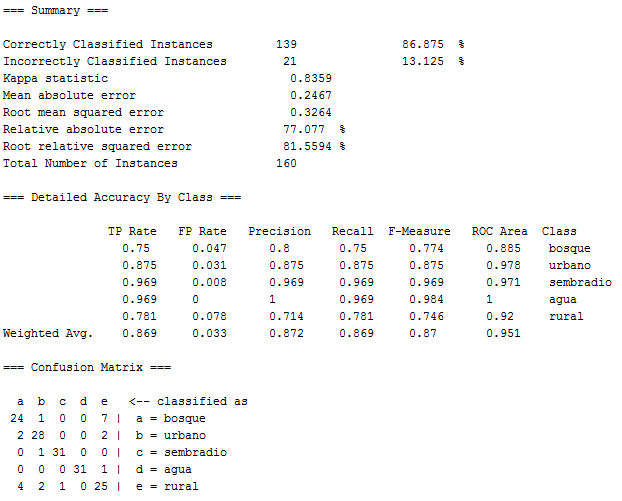
\includegraphics[width=1\textwidth]{images/salida-SMO.png}
    \caption{Fragmento de la salida de un clasificador SMO en Weka. Se pueden identificar datos importantes como el número y porcentaje de instancias clasificadas correcta e incorrectamente, la matriz de confusión y un bloque detallando la precisión por categoria.}
    \label{fig:salida-SMO}
\end{figure}

\subsection{Cálculo de Precisión}

La métrica de precisión que se utilizó para medir el desempeño de este experimento fue provista por el mismo Weka. El estadístico \textit{correctly classified instances} muestra tanto la cantidad de imágenes clasificadas correctamente así como un porcentaje. Este valor se calcula utilizando la matriz de confusión, como se muestra en la siguiente función:

\begin{equation}
  \text{Precisión} = \cfrac{ M_{1,1} + M_{2,2} + ... + M_{n,n}}{\text{Total de instancias}}
\end{equation}
Donde:
\begin{itemize}
    \item $M$ es la matriz de confusión.
    \item $n$ es el total de categorías, en este caso tipos de cobertura.
\end{itemize}
  

\subsection{Clasificadores}

Se seleccionaron cuatro clasificadores para evaluar la precisión. Cada uno tiene una naturaleza distinta: agrupamiento, basado en funciones, regresión y teoría Bayesiana. A continuación se describen cada uno de los clasificadores.


\subsubsection{K-Means}

El primer clasificador es un algoritmo básico de agrupamiento (o \textit{clustering} en inglés), llamado \textbf{K-Means}\cite{MacQueen1967}.

A grandes rasgos, este algoritmo interpreta cada arreglo de TF como un vector euclidiano en un espacio $n$-dimensional. Sobre este espacio se lanzan $k$ puntos, los \textit{centroides}, de manera aleatoria. 
Posteriormente, se hacen $i$ iteraciones en las cuales se miden los vectores más cercanos a cada centroide el cual se reposiciona hacia el centro de los vectores cercanos.
La idea es que luego de varias pasadas, los centroides irán gravitando hacia el centro de las nubes de puntos que representan las categorías (en este caso imágenes).

En Weka, la implementación de K-Means se denomina ``simpleKMeans''. Los parámetros de ejecución fueron:
\begin{itemize}
    \item Uso de todo el conjunto de datos para entrenamiento.
    \item 500 iteraciones.
    \item Uso de distancia euclidiana para el cálculo de cercanía.
\end{itemize}


\subsubsection{Máquina de Soporte Vectorial}

El segundo clasificador es un algoritmo de aprendizaje automático llamado \textbf{Máquina de Soporte Vectorial} (o \textit{Support Vector Machine} en inglés), en este caso particular usando el algoritmo de Optimización Secuencial Mínima\cite{Platt1999} (SMO por sus siglas en inglés).
Las Máquinas de Soporte Vectorial se utilizan normalmente en datos con alta dimensionalidad. Aquí, los datos se intentan dividir (clasificar) por medio de un hiperplano. Este plano no siempre existe por lo que los datos son transformados por una función no lineal llamada \textit{kernel} con el fin de facilitar su determinación.
En Weka, este algoritmo se denomina ``SMO'' y sus parámetros de ejecución fueron:
\begin{itemize}
    \item Entrenamiento usando Validación Cruzada de 10 iteraciones. Esta técnica se muestra en la figura \ref{fig:cross-validation}.
    \item Función \textit{Kernel} polinomial.
    \item Error aceptable de $1.0 \times 10^{-12}$.
    \item Normalización de los datos.
\end{itemize}

\begin{figure}
    \centering
    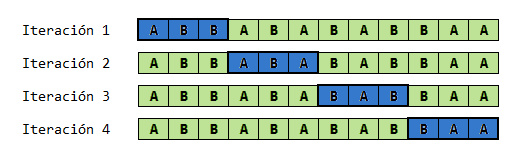
\includegraphics[width=0.75\textwidth]{images/cross-validation.png}
    \caption{Técnica de Validación Cruzada de 4 iteraciones. El conjunto de datos está compuesto por ítemes de los grupos A y B. En cada iteración, el grupo de elementos en azul se usa para validación y el grupo en verde para entrenamiento. Estos grupos van rotando tantas veces como iteraciones se dispongan.}
    \label{fig:cross-validation}
\end{figure}


\subsubsection{Regresión}

El siguiente clasificador sigue un modelo aditivo generalizado, (o \emph{boosting} en inglés). 
Esta técnica transforma un algoritmo débil en uno robusto al aplicarlo en sucesiones e ir ajustando una serie de pesos a lo largo de cada iteración. 
El algoritmo debil utilizado en este caso es la clásica técnica estadística de regresión, particularmente la regresión logística. La implementación de esta técnica se denomina \textbf{LogitBoost}\cite{Friedman2000}. En Weka se conoce con el mismo nombre y se utilizó con los parámetros por defecto.


\subsubsection{Redes bayesianas}

El último clasificador es el algoritmo de \textbf{red bayesiana}\cite{Bouckaert2008}. Las redes bayesianas son un modelo probabilístico que representa un conjunto de variables aleatorias y las condiciones de sus dependencias a través de un grafo dirigido cuyas aristas son probabilidades de que,  dada una variable, se dé otra. En el caso de la TT, se debe entender cada TF como una variable aleatoria y la red bayesiana intenta mapear las dependencias entre cada TF con el fin de maximizar la probabilidad de que todo el vector corresponda con la imagen original.
En Weka se denomina ``BayesNet'' y se usó con los parámetros por defecto.



\chapter{Resultados y análisis} 

Los datos experimentales se analizaron por medio de ANOVA, donde los grupos estudiados para el experimento A son la combinación de cada uno de los factores como muestra el cuadro \ref{tab:gruposA}.\\

\begingroup
\renewcommand\arraystretch{0.75}
\begin{longtable}{|c|c|c|c|}

        \hline
        \textbf{$\Delta \tau$ (píxeles)} & \textbf{$\Delta \rho$ (píxeles)} & \textbf{$\Delta \phi$ (grados)} & \textbf{Cobertura} \\ 
        \hline
        \endhead
        1 & 1 & 0,5 & Agua \\ \hline
        1 & 1 & 0,5 & Bosque \\ \hline
        1 & 1 & 0,5 & Urbano \\ \hline
        ... & ... & ... & ... \\ \hline
        1 & 1 & 1 & Agua \\ \hline
        1 & 1 & 1 & Bosque \\ \hline
        ... & ... & ... & ... \\ \hline
        1 & 1 & 2 & Agua \\ \hline
        1 & 1 & 2 & Bosque \\ \hline
        ... & ... & ... & ... \\ \hline
        3 & 3 & 2 & Urbano \\ \hline
        
    
    \caption{Grupos estudiados en el experimento A.}
    \label{tab:gruposA}
\end{longtable}
\endgroup

%\begin{itemize}
    %\item $\Delta\tau$=1-$\Delta\rho$=1-$\Delta\phi$=1-Cobertura=Agua
    %\item $\Delta\tau$=1-$\Delta\rho$=1-$\Delta\phi$=1-Cobertura=Bosque
    %\item ... 
    %\item $\Delta\tau$=3-$\Delta\rho$=3-$\Delta\phi$=2-Cobertura=Urbano
%\end{itemize}

Para el experimento B, los grupos estudiados fueron se presentan en el cuadro \ref{tab:gruposB}.\\

\begingroup
\renewcommand\arraystretch{0.75}
\begin{longtable}{|c|c|c|c|}
        \hline
        \textbf{$\Delta \tau$ (píxeles)} & \textbf{$\Delta \rho$ (píxeles)} & \textbf{$\Delta \phi$ (grados)} & \textbf{Clasificador} \\  
        \hline
        \endhead
        1 & 1 & 0,5 & K-Means \\ \hline
        1 & 1 & 0,5 & SMO \\ \hline
        1 & 1 & 0,5 & LogitBoost \\ \hline
        ... & ... & ... & ... \\ \hline
        1 & 1 & 1 & K-Means \\ \hline
        1 & 1 & 1 & SMO \\ \hline
        ... & ... & ... & ... \\ \hline
        1 & 1 & 2 & K-Means \\ \hline
        1 & 1 & 2 & SMO \\ \hline
        ... & ... & ... & ... \\ \hline
        3 & 3 & 2 & BayesNet \\ \hline
        
    
    \caption{Grupos estudiados en el experimento B.}
    \label{tab:gruposB}
\end{longtable}
\endgroup

%\begin{itemize}
    %\item $\Delta\tau$=1-$\Delta\rho$=1-$\Delta\phi$=1-Clasificador=K-Means
    %\item $\Delta\tau$=1-$\Delta\rho$=1-$\Delta\phi$=1-Clasificador=SMO
    %\item ... 
    %\item $\Delta\tau$=3-$\Delta\rho$=3-$\Delta\phi$=2-Clasificador=BayesNet
%\end{itemize}

Para poder utilizar ANOVA es necesario validar una serie de supuestos\cite{Montgomery2001}, que en caso de no hacerlo, no se puede asegurar la validez del procedimiento. Estos supuestos son:
\begin{enumerate}
    \item \textbf{Independencia y aleatoriedad} de las observaciones: esto se valida con el diseño experimental, donde se muestra que cada corrida del experimento A y B es independiente de cualquier otra. Este supuesto se aseguró al ejecutar una sola extracción por nodo y al ejecutar las extracciones de manera aleatoria.
    \item \textbf{Normalidad} de los residuos: Esto se puede verificar con la prueba de Lilliefors (Kolmogorov-Smirnov)\cite{Thode2002} o de manera visual con un gráfico de cuantiles contra cuantiles (Q-Q en ingés). Para la prueba, el estadístico $D$ debe ser menor que el valor-p para confirmar normalidad. En el gráfico Q-Q, se gráfican los residuos estandarizados de la variable medida por cuantiles contra los cuantiles teóricos de la variable de respuesta y una línea de tendencia, mientras más se alejen los puntos de esta línea, menos normales son los datos.
    \item \textbf{Homogeneidad} de varianzas (homocedasticidad): Esto se puede verificar con la prueba de Levene\cite{Levene1960} o de manera visual con un gráfico de residuos contra valores ajustados (RvVA) de ANOVA. Para la prueba, el estadístico $W$ debe ser menor que el valor-p para confirmar homogeneidad. En el gráfico, los puntos deben estar dispersos y no seguir algún patrón fácilmente reconocible, en caso contrario, los datos no son homocedásticos.
\end{enumerate}

El paquete estadístico R\footnote{\url{http://www.r-project.org/}} se utilizó para todo el análisis siguiente.

\section{Experimento A}

\subsection{Verificación de supuestos}

Para los datos de tiempo recolectados en el experimento A, se utilizó la verificación visual inicialmente. En la figura \ref{fig:sin-transformacion} se muestra el gráfico Q-Q y el gráfico RvVA. En ambos gráficos se puede notar como los supuestos no se cumplen; los puntos se alejan de forma variable en un patrón de S de la línea de tendencia para la normalidad y se nota un patrón de cono y varios cúmulos de puntos en el gráfico de la homogeneidad.
Para confirmar estas hipótesis se ejecutaron las pruebas estadísticas para normalidad y homogeneidad, que confirmaron lo observado en los gráficos. El resultado de la prueba de Lilliefors se muestra en la figura \ref{fig:lillie-t} y el resultado de la prueba de Levene en la figura \ref{fig:levene-t}.
En ambos casos el estadístico calculado descarta ambos supuestos.


\begin{figure}[H]
    \centering
    \subfigure[Cuantiles contra Cuantiles]{
        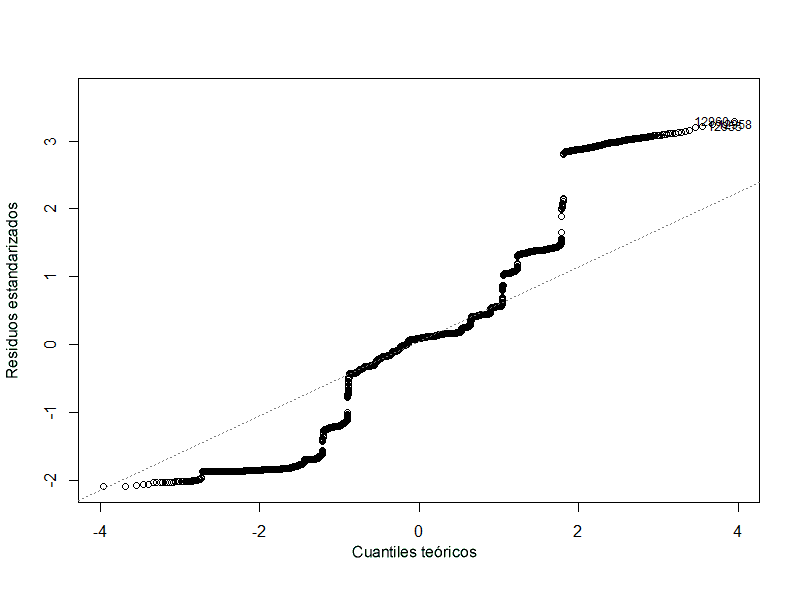
\includegraphics[width=.75\textwidth]{images/t/qq-t.png}
    }
    \subfigure[Residuos contra Valores Ajustados]{
        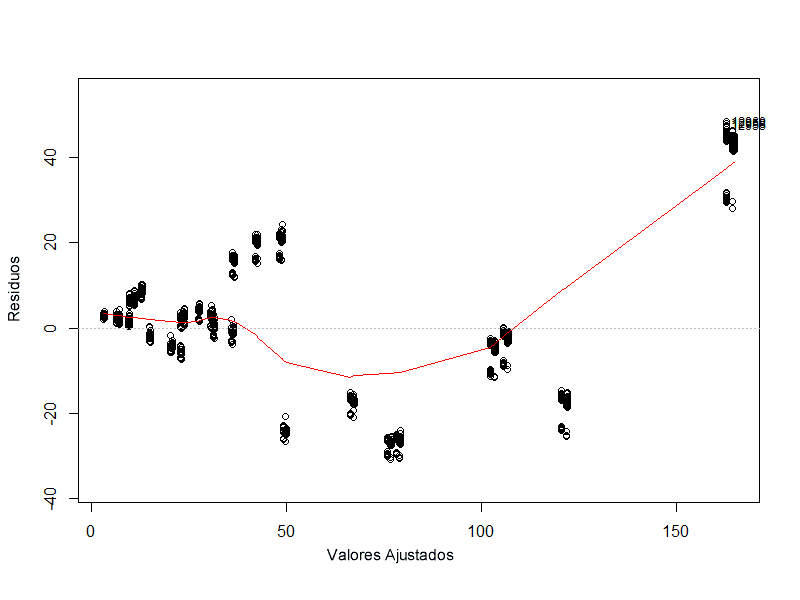
\includegraphics[width=.75\textwidth]{images/t/rvf-t.png}
    }
    \caption{Exploración visual de la normalidad y homogeneidad de varianza en los datos de tiempo sin transformaciones.}
    \label{fig:sin-transformacion}
\end{figure}


\begin{figure}[H]
    \centering
        \small{
        \begin{alltt}
        
        
            > lillie.test(data-t)
                Lilliefors (Kolmogorov-Smirnov) normality test
            data:  data-t
            D = 0.2085, p-value < 2.2e-16
        \end{alltt}
        }
    
    \caption{Prueba de Lilliefors para normalidad en R. El estadístico es mayor que el valor-p por lo que los datos no son normales.}
    \label{fig:lillie-t}
\end{figure}

\begin{figure}[H]
    \centering
        \small{
        \begin{alltt}
        
        
            > levene.test(data-t, data-grupo)
                modified robust Brown-Forsythe Levene-type test 
                based on the absolute deviations from the median
            data:  data-t
            Test Statistic = 21.8013, p-value < 2.2e-16
        \end{alltt}
        }
    \caption{Prueba de Levene para homogeneidad de varianzas en R. El estadístico es mayor que el valor-p por lo que los datos no tiene varianzas homogéneas.}
    \label{fig:levene-t}
\end{figure}




Según \cite{Montgomery2001} en el caso de que los supuestos de ANOVA no se cumplan se pueden tomar varios caminos:
\begin{enumerate}
    \item Aplicar transformaciones a los datos para que cumplan los supuestos y hacer un análisis basado en los nuevos datos.
    \item Utilizar un Modelo Lineal Generalizado.
    \item Usar el método Box-Cox.
    
\end{enumerate}

Todas las estrategias se siguieron y fallaron. A continuación, se presentara el detalle de cada una y la solución final, que consistía en hacer una transformación por rangos\cite{SAS2004}.

%Todas las estrategias se siguieron y fallaron. A continuación, se presentara el detalle de cada una y la solución final, que fue consultada con una experta en estadística de la Unidad de Servicios en Estadística\footnote{\url{http://www.estadistica.ucr.ac.cr/contenido/uses/}} (USES) de la Escuela de Estadística de la Universidad de Costa Rica y que consistía en hacer una transformación por rangos, o que hace que los supuestos de ANOVA se puedan descartar\cite{SAS2004}.

\subsubsection{Transformaciones}

Según la literatura, se pueden aplicar transformaciones según se vea conveniente. Para este caso, se aplicaron las transformaciones de potencia $e$, raíz cuadrada y logaritmo base 10. Estas son las más comunes y a su vez las que tienen más sentido a la hora de la interpretación de los nuevos datos transformados: una transformación de potencia o logaritmo amplía o reduce la distancia de los puntos más altos, en este caso, los tiempos de mayor duración. Es mucho más complejo interpretar una transformación como la siguiente:
\begin{equation}
t-transformado = (t + 24)^2 - sen(2*\pi * t)
\end{equation}

Desgraciadamente ninguna de éstas transformaciones normalizó o cumplió la homogeneidad de varianzas, la exploración visual se hizo como al inicio y reveló los \textbf{mismos problemas}. Las figuras \ref{fig:transformacion-e}, \ref{fig:transformacion-log} y \ref{fig:transformacion-sqrt} muestran los gráficos Q-Q y RvVA de estas transformaciones. En todos los gráficos Q-Q se nota como los puntos se alejan de la línea de tendencia. Los gráficos RvAF también tiene patrones bien marcados, de conos o cúmulos de puntos.



\begin{figure}[H]
\centering
    \subfigure[Cuantiles contra Cuantiles de la Transformación con potencia $e$.]{
        \centering
        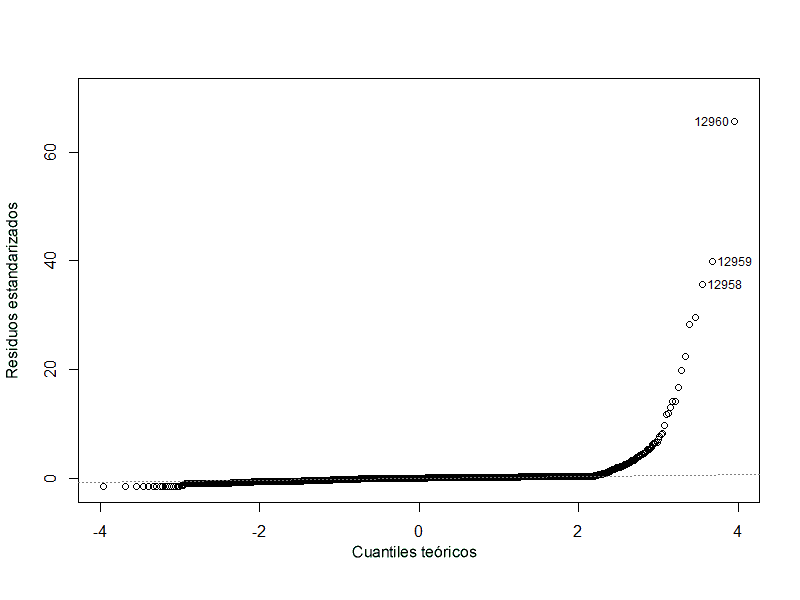
\includegraphics[width=0.75\textwidth]{images/t/qq-e.png}
    }
    \subfigure[Residuos contra Valores Ajustados de la Transformación con potencia $e$.]{
        \centering
        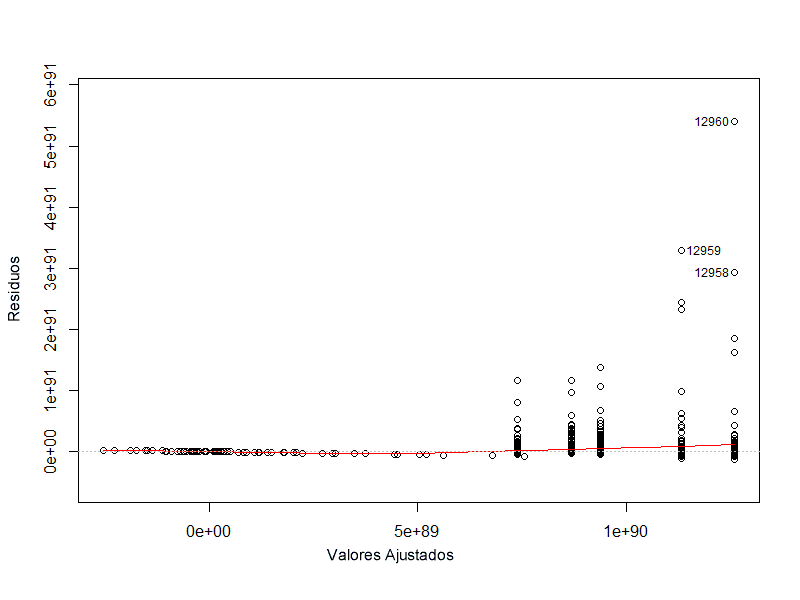
\includegraphics[width=0.75\textwidth]{images/t/rvf-e.png}
    }
\caption{Exploración visual de la normalidad y homogeneidad de varianza en los datos de tiempo transformados con una potencia $e$.}
\label{fig:transformacion-e}
\end{figure}


\begin{figure}[H]
\centering
    \subfigure[Cuantiles contra Cuantiles de la Transformación con logaritmo base 10.]{
        \centering
        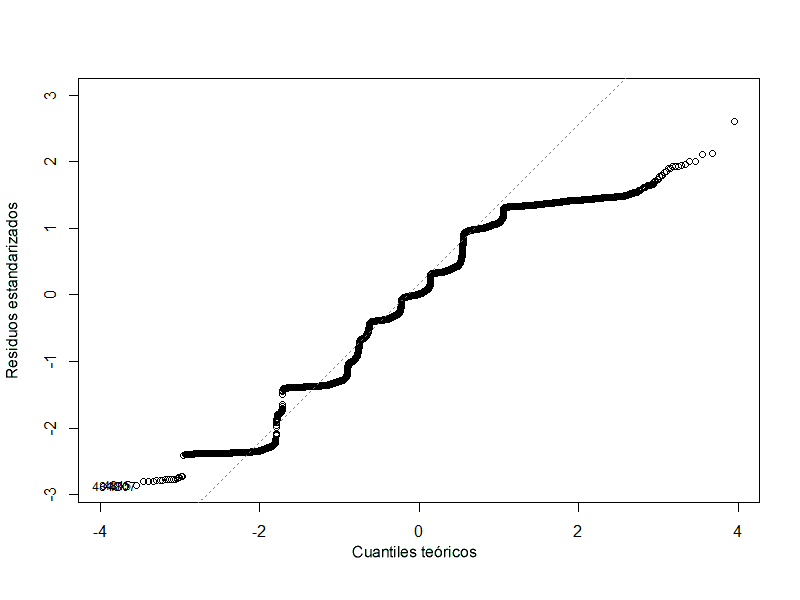
\includegraphics[width=0.75\textwidth]{images/t/qq-log.png}
    }
    \subfigure[Residuos contra Valores Ajustados de la Transformación con logaritmo base 10.]{
        \centering
        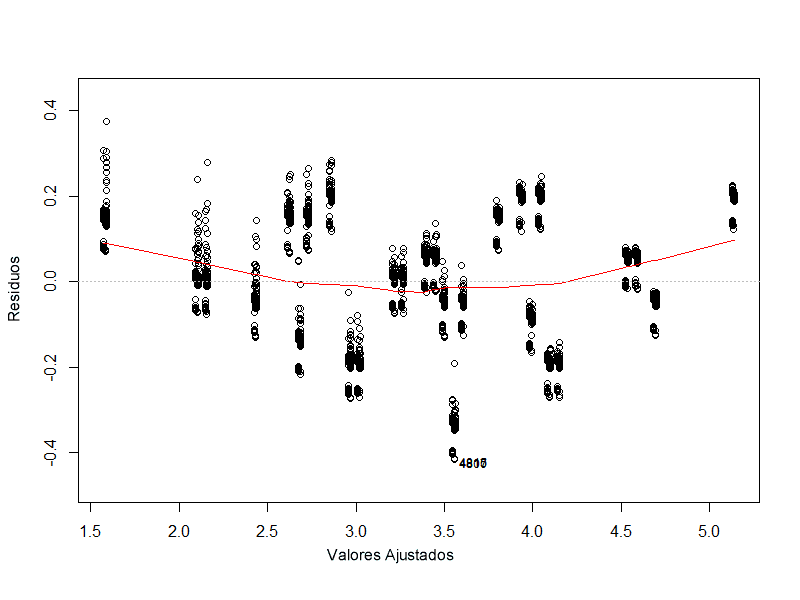
\includegraphics[width=0.75\textwidth]{images/t/rvf-log.png}
    }
\caption{Exploración visual de la normalidad y homogeneidad de varianza en los datos de tiempo transformados con una logaritmo base 10.}
\label{fig:transformacion-log}
\end{figure}


\begin{figure}[H]
\centering
    \subfigure[Cuantiles contra Cuantiles de la Transformación con raíz cuadrada.]{
        \centering
        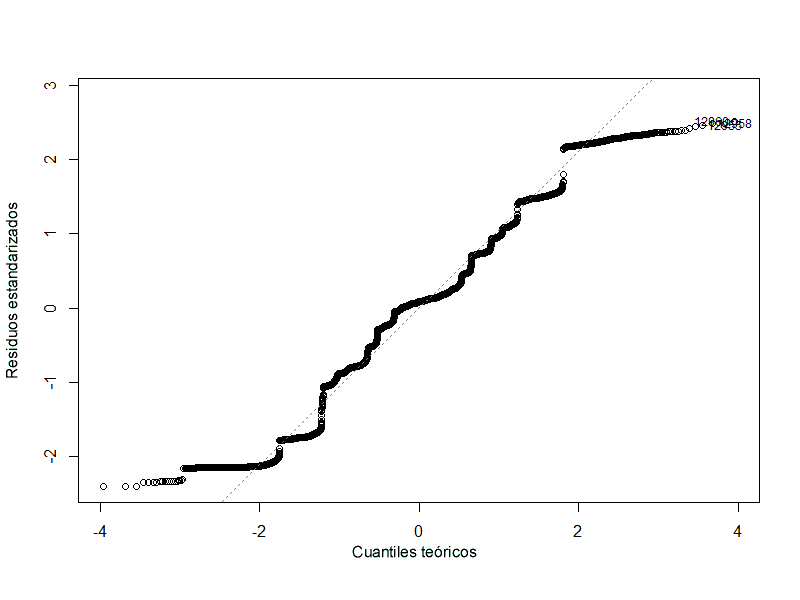
\includegraphics[width=0.75\textwidth]{images/t/qq-sqrt.png}
    }
    \subfigure[Residuos contra Valores Ajustados de la Transformación con raíz cuadrada.]{
        \centering
        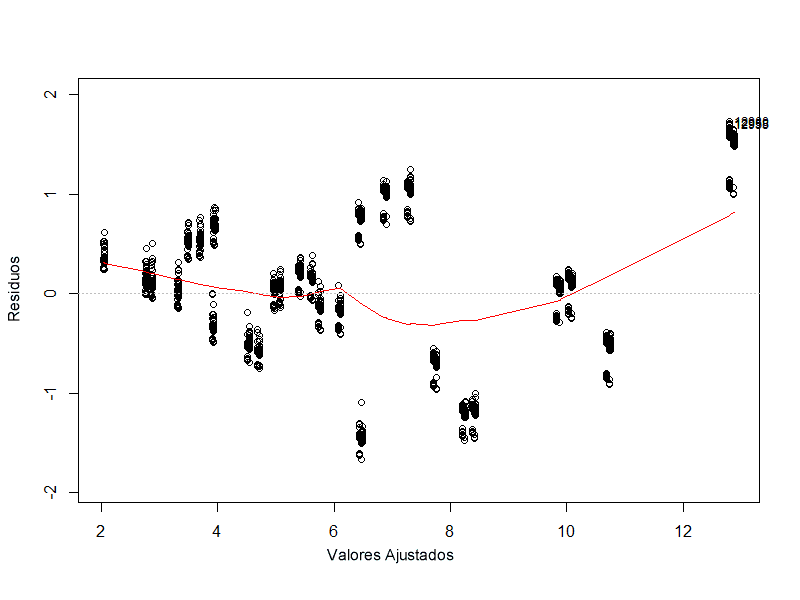
\includegraphics[width=0.75\textwidth]{images/t/rvf-sqrt.png}
    }
\caption{Exploración visual de la normalidad y homogeneidad de varianza en los datos de tiempo transformados con una raíz cuadrada.}
\label{fig:transformacion-sqrt}
\end{figure}

\subsubsection{Modelo Lineal Generalizado}

El Modelo Lineal Generalizado (GLM por sus siglas en inglés) es una generalización de la regresión lineal, que no toma como un hecho la distribución gaussiana del error en la variable de respuesta\cite{Montgomery2001}.

Para utilizar un GLM se necesita:
\begin{itemize}
    \item Una función de enlace.
    \item Una distribución de probabilidad para los errores.
\end{itemize}

La escogencia de estos dos requerimientos hace que nuevamente se hagan supuestos sobre los datos y debido a esto, se descartó.


\subsubsection{Método Box-Cox}

El método Box-Cox\cite{Sakia1992} es una función de optimización, donde se minimiza la desviación estándar de un conjunto de datos al calcular una transformación de potencia $\lambda$.
La figura \ref{fig:box-cox} muestra el resultado del proceso Box-Cox en R, donde se puede notar que la transformación óptima es cerca de $-1$.


\begin{figure}[H]
    \centering
    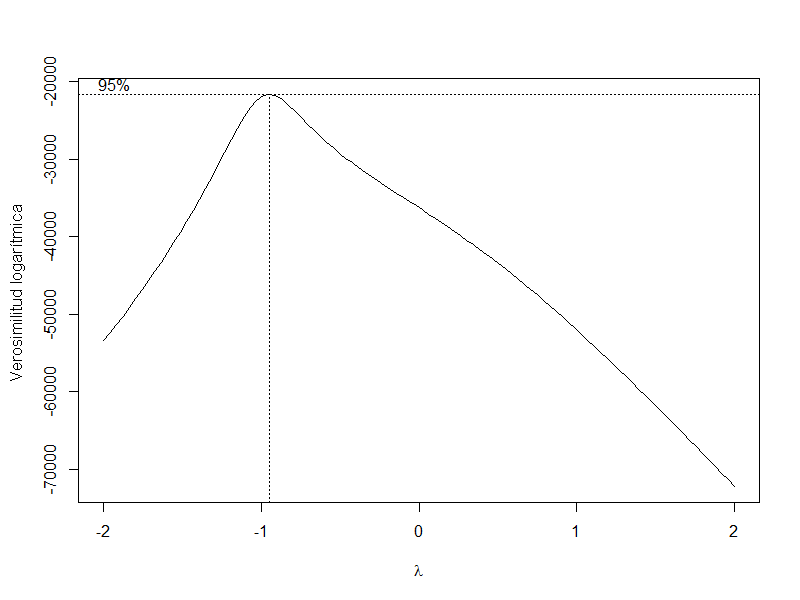
\includegraphics[width=0.75\textwidth]{images/t/box-cox.png}
    \caption{Método Box-Cox. El punto óptimo $\lambda$, con un 95\% de confianza se encuentra cerca de -1.}
    \label{fig:box-cox}
\end{figure}


Al aplicar una transformación de potencia $-1$, la exploración visual nuevamente falla al validar los supuestos de ANOVA. La figura \ref{fig:transformacion-bc} muestra el gráfico Q-Q y RvAF de la transformación sugerida por el método Box-Cox.

\begin{figure}[H]
\centering
    \subfigure[Cuantiles contra Cuantiles de la Transformación con el método Box-Cox.]{
        \centering
        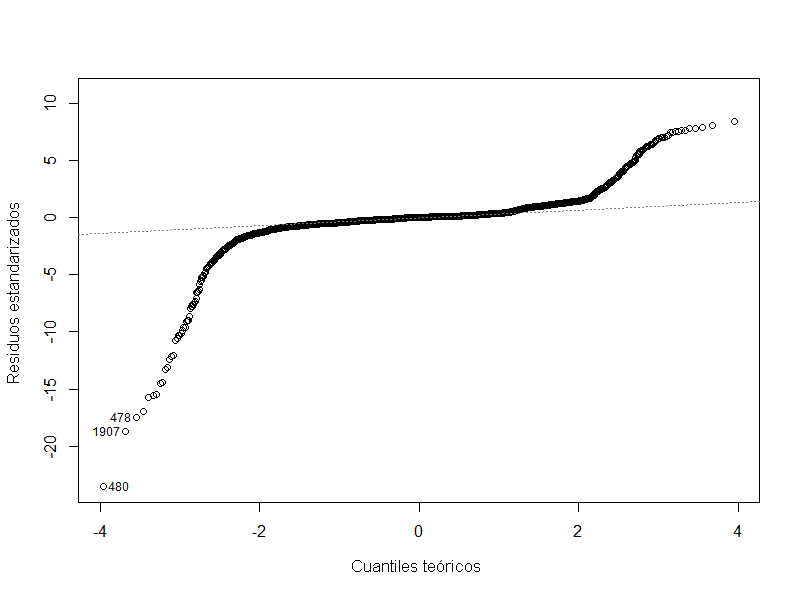
\includegraphics[width=0.75\textwidth]{images/t/qq-bc.png}
    }
    \subfigure[Residuos contra Valores Ajustados de la Transformación con el método Box-Cox.]{
        \centering
        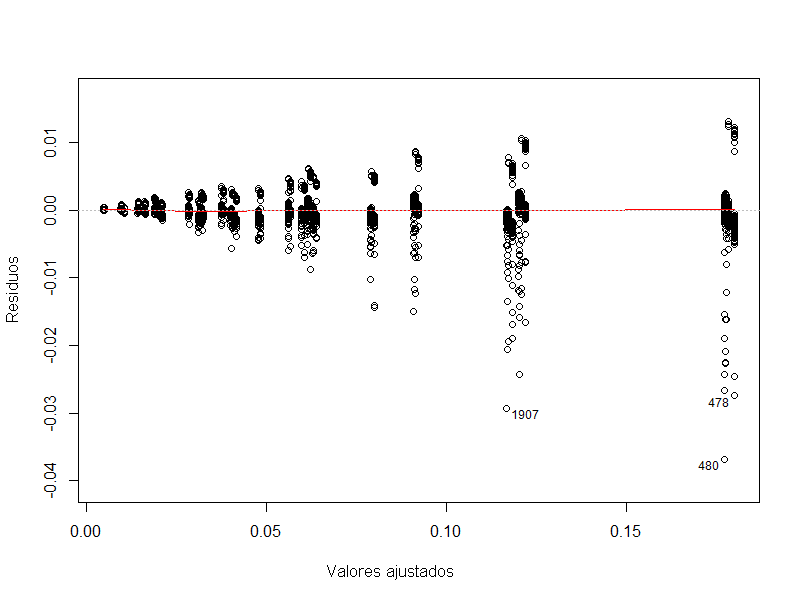
\includegraphics[width=0.75\textwidth]{images/t/rvf-bc.png}
    }
\caption{Exploración visual de la normalidad y homogeneidad de varianza en los datos de tiempo transformados con el método Box-Cox.}
\label{fig:transformacion-bc}
\end{figure}


\subsubsection{Transformación por Rangos}

Luego de haber agotado las opciones brindadas por la literatura, se decidió consultar a la USES, donde se concertaron dos reuniones de trabajo donde se decidió por criterio experto hacer una transformación por Rangos, que elimina los supuestos de ANOVA\cite{USES2014}\cite{SAS2004}.

La transformación por rangos es un proceso estadístico que toma el mejor valor de una variable y le asigna el rango de 1, toma el siguiente mejor valor y asigna el rango de 2 sucesivamente hasta el peor valor de la variable y se le asigna el ultimo rango. 

Para los tiempos en la TT, un tiempo bajo es un buen valor y un tiempo alto es un valor malo, así, el tiempo de 5,177 segundos tiene el rango 1 y el tiempo de 216,606 segundos, el rango 12960. Esta conversión sigue la función en la gráfica de la figura \ref{fig:rank-t}.

\begin{figure}[H]
    \centering
    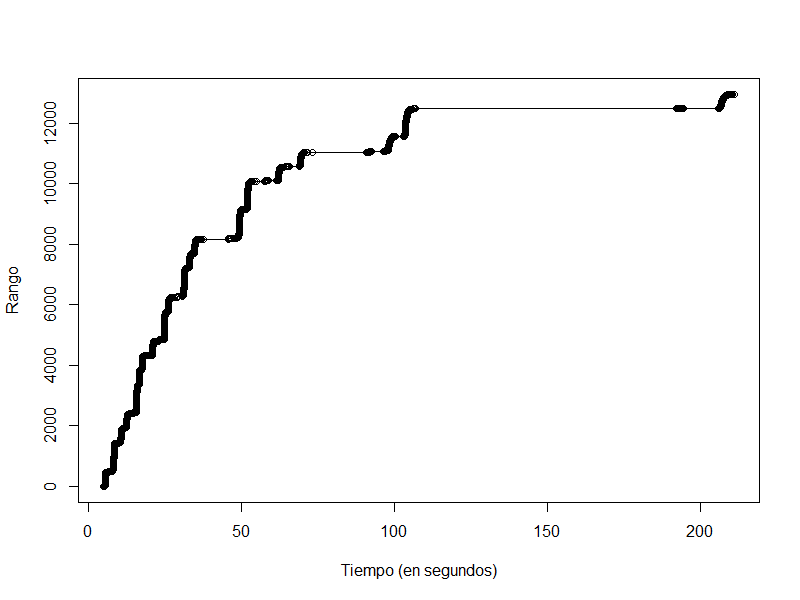
\includegraphics[width=0.75\textwidth]{images/t/rank.png}
    \caption{Transformación por rangos de los datos de tiempo tomados en el experimento A.}
    \label{fig:rank-t}
\end{figure}

\subsection{Análisis de resultados}

Una vez superado los supuestos de ANOVA, se procedió a hacer el análisis de los tiempos transformados a rangos.

El procedimiento \texttt{aov} en R es el utilizado para hacer el análisis de varianza. Esta función reporta dos salidas: una tabla de ANOVA y el cuadro resumen, de los cuales la tabla es la que nos interesa.

La figura \ref{fig:anova-t} muestra la invocación de la función \texttt{aov} y la tabla \ref{tab:anovaA} muestra la relevancia de cada combinación de factores.

\begin{figure}[H]
    \centering
            \small
            \begin{alltt}
            
            
            > aov(rank(t) ~ dTau * dRho * dPhi * cobertura)
            \end{alltt}
    \caption{Invocación de la función aov para Análisis de Varianza en R. El parámetro recibido muestra las relaciones entre las variables: $rank(t)$ la variable de respuesta se debe analizar en función de $\Delta \tau$, $\Delta \rho$, $\Delta \phi$, tipo de cobertura y todas sus combinaciones.}
    \label{fig:anova-t}
\end{figure}


\begin{table}\renewcommand{\tabcolsep}{3pt}
    \centering
    \small
    \begin{tabular}{lrrrrrr}
        \hline 
        Factor & Df & Sum Sq & Mean Sq & F-value & Pr($>$F) & Sig.\\
        \hline 
        \textbf{dTau} & 1 & 6.056e+10 & 6.056e+10 & 9.681e+04 & $<$2e-16 & 0\\
        \textbf{dPhi} & 1 & 7.188e+10 & 7.188e+10 & 1.149e+05 & $<$2e-16 & 0\\
        \textbf{dRho} & 1 & 3.796e+10 & 3.796e+10 & 6.068e+04 & $<$2e-16 & 0\\
        \textbf{cobertura} & 4 & 2.135e+07 & 5.338e+06 & 8.533e+00 & 7.15e-07 & 0\\
        \textbf{dTau:dPhi} & 1 & 5.291e+07 & 5.291e+07 & 8.458e+01 & $<$2e-16 & 0\\
        \textbf{dTau:dRho} & 1 & 1.383e+08 & 1.383e+08 & 2.211e+02 & $<$2e-16 & 0\\
        dPhi:dRho & 1 & 1.108e+03 & 1.108e+03 & 2.000e-03 & 0.966 & \\
        dTau:cobertura & 4 & 2.380e+06 & 5.951e+05 & 9.510e-01 & 0.433 & \\
        dPhi:cobertura & 4 & 8.064e+04 & 2.016e+04 & 3.200e-02 & 0.998 & \\
        dRho:cobertura & 4 & 1.340e+05 & 3.351e+04 & 5.400e-02 & 0.995 & \\
        \textbf{dTau:dPhi:dRho} & 1 & 2.709e+09 & 2.709e+09 & 4.330e+03 & $<$2e-16 & 0\\
        dTau:dPhi:cobertura & 4 & 1.172e+06 & 2.929e+05 & 4.680e-01 & 0.759 & \\
        dTau:dRho:cobertura & 4 & 6.292e+04 & 1.573e+04 & 2.500e-02 & 0.999 & \\
        dPhi:dRho:cobertura & 4 & 8.207e+05 & 2.052e+05 & 3.280e-01 & 0.859 & \\
        dTau:dPhi:dRho:cobertura & 4 & 4.000e+05 & 1.000e+05 & 1.600e-01 & 0.959 &\\
        Residuos & 12920 & 8.082e+09 & 6.256e+05\\
        \hline
    \end{tabular}
    \caption{Tabla ANOVA para los rangos de tiempo del experimento A.}
    \label{tab:anovaA}
\end{table}

La tabla indica que existen siete combinaciones de factores que influyen sobre la variable de respuesta. Estos son los cuatro factores principales, las interacción de segundo nivel $\Delta \tau$ con $\Delta \rho$ y $\Delta \tau$ con $\Delta \phi$, y la interacción de tercer nivel de los parámetros de frecuencia.

El efecto de los factores principales se evidencia en la figura \ref{tab:ME-A}. Todos los parámetros de frecuencia muestran un decremento en tiempo mientras más crecen (un rango alto representa un tiempo largo), lo que es esperable: \textbf{a más fino el barrido, más tiempo se tarda extraer las características}. 

\begin{figure}[H]
    \centering
    \subfigure[$\Delta \tau$]{
    	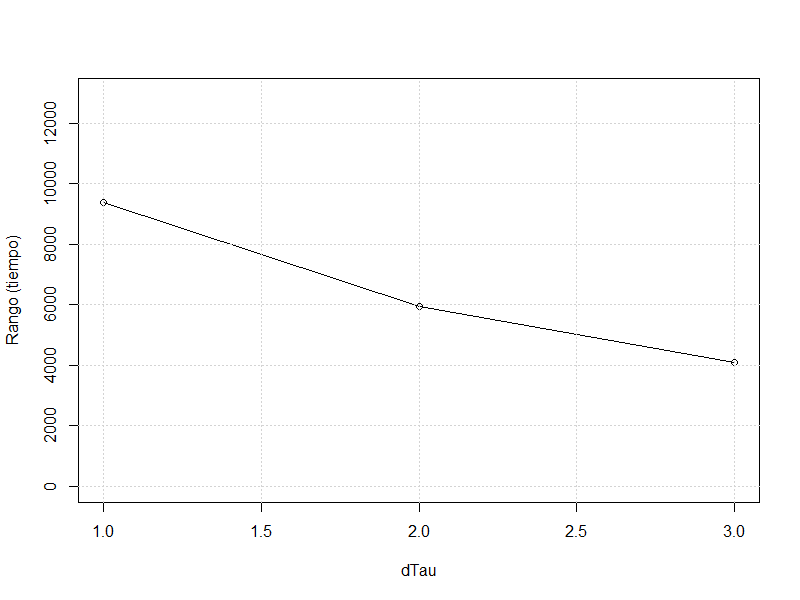
\includegraphics[width=0.4\textwidth]{images/t/t-MEdTau.png}
    }
    \subfigure[$\Delta \rho$]{
         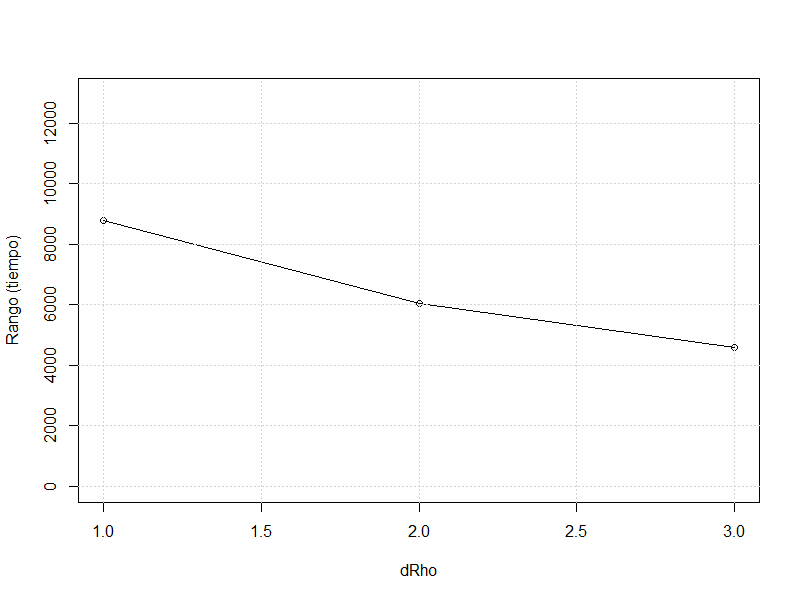
\includegraphics[width=0.4\textwidth]{images/t/t-MEdRho.png}
    }
    \subfigure[$\Delta \phi$]{
        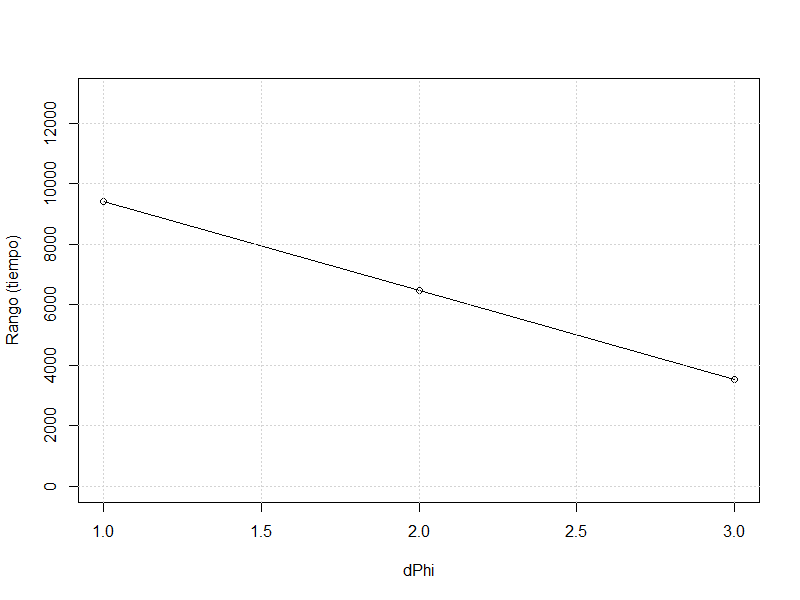
\includegraphics[width=0.4\textwidth]{images/t/t-MEdPhi.png}
    }
    \subfigure[Tipo de cobertura de terreno]{
        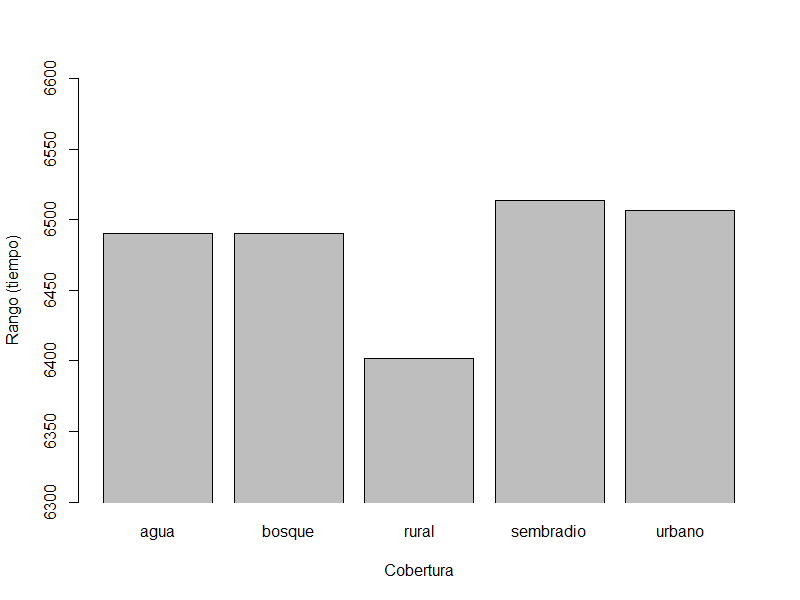
\includegraphics[width=0.4\textwidth]{images/t/t-MEcobertura.png}
    }
\caption{Promedio del efecto de los factores principales del experimento A.}
\label{tab:ME-A}
\end{figure}

El efecto que tiene el tipo de cobertura sobre el tiempo es poco, pero dado el análisis, es significativo. El tipo de cobertura rural, aunque muestre un mejor tiempo en promedio, la diferencia es ínfima: del rango 6400 al 6500 la diferencia es de 0,03033333 segundos.

Las interacciones de segundo nivel se muestran en la figura \ref{tab:2I-A}. La subfigura (a) expone el promedio de los rangos cuando $\Delta \tau$ y $\Delta \phi$ cambian juntos, de igual manera pero con $\Delta \rho$ en la subfigura (b). 

\begin{figure}[H]

    \centering
    \subfigure[$\Delta \tau$ y $\Delta \phi$]{
    	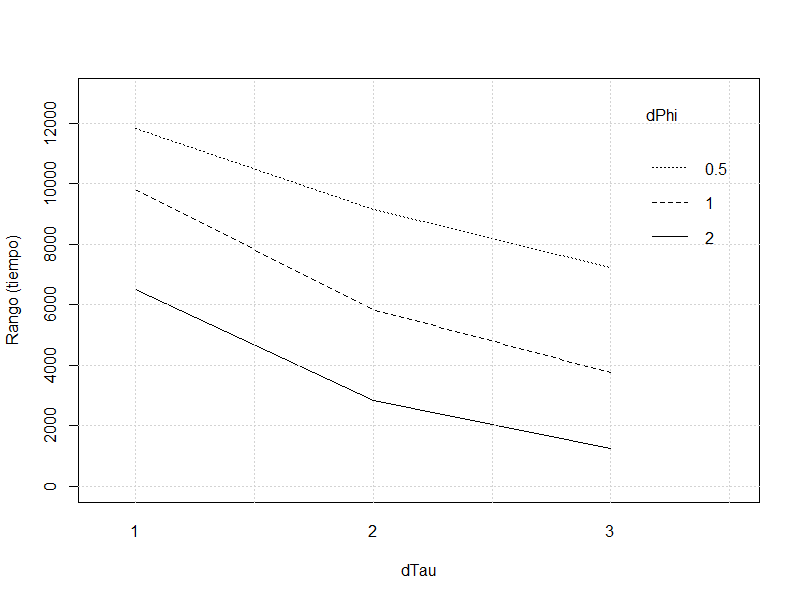
\includegraphics[width=0.75\textwidth]{images/t/t-2IdTau-dPhi.png}
    }
    \subfigure[$\Delta \tau$ y $\Delta \rho$]{
        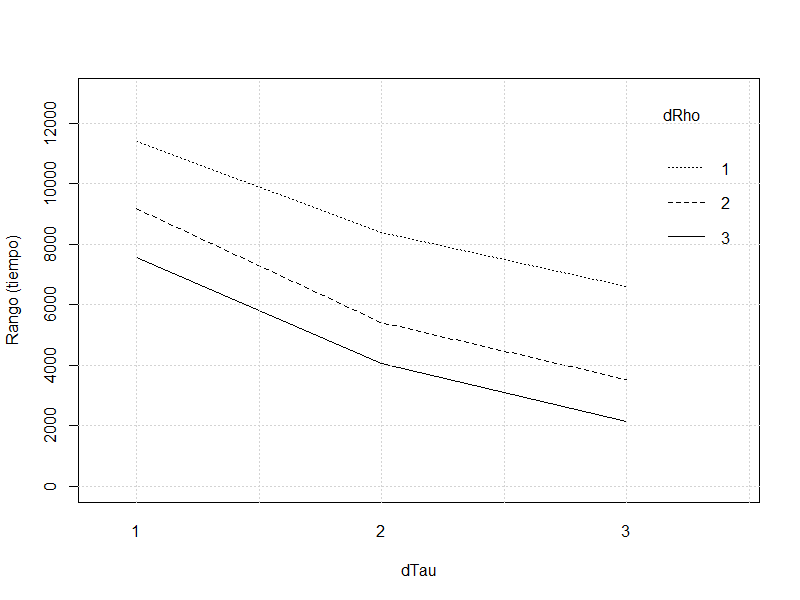
\includegraphics[width=0.75\textwidth]{images/t/t-2IdTau-dRho.png}
    }
\caption{Promedio de interacciones de segundo nivel en el experimento A.}
\label{tab:2I-A}
\end{figure}

En ambos, se muestra un comportamiento decreciente en los rangos y tiempos a como se incrementan los parámetros de frecuencia, siendo los puntos extremos nuevamente las combinaciones $\Delta \tau=3$, $\Delta \phi=2$ y $\Delta \tau=3$, $\Delta \rho=3$. El efecto es ligeramente más marcado con $\Delta \phi$, donde los rangos son más bajos.

Por último, la interacción de tercer nivel se muestra en la figura \ref{tab:3I-A}. Esta interacción toma en cuenta todas las variaciones de los parámetros de frecuencia y deja por fuera el tipo de cobertura de terreno.

En todos los casos el comportamiento no es una sorpresa,  es decreciente en bloques: con $\Delta \tau=1$ se tarda más en promedio, con cualquier valor de $\Delta \rho$ y $\Delta \phi$, que con $\Delta \tau=3$. Esto significa, que al igual que como se indican con las interacciones anteriores, el tiempo de extracción decrece a como los parámetros aumentan ya sea de manera independiente o conjunta.



\begin{figure}[H]
    \centering
    \subfigure[$\Delta \tau$=1 y $\Delta \rho$ y $\Delta \phi$]{
    	
		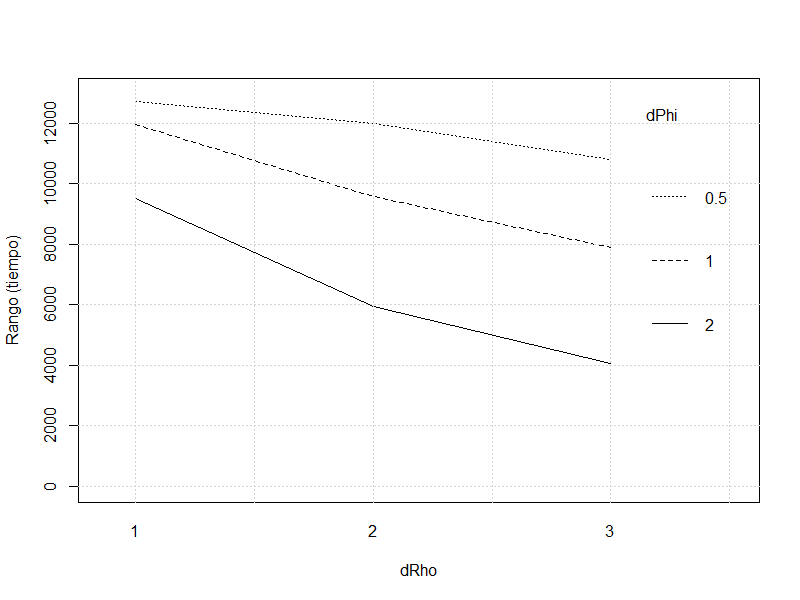
\includegraphics[width=0.5\textwidth]{images/t/t-3I-t1.png}
    }
    \subfigure[$\Delta \tau$=2 y $\Delta \rho$ y $\Delta \phi$]{
        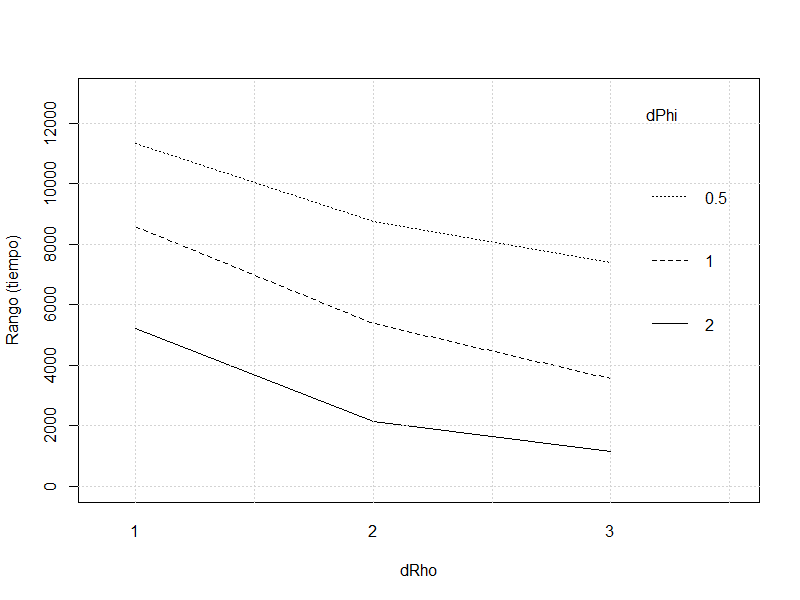
\includegraphics[width=0.5\textwidth]{images/t/t-3I-t2.png}
    }
    \subfigure[$\Delta \tau$=3 y $\Delta \rho$ y $\Delta \phi$]{
        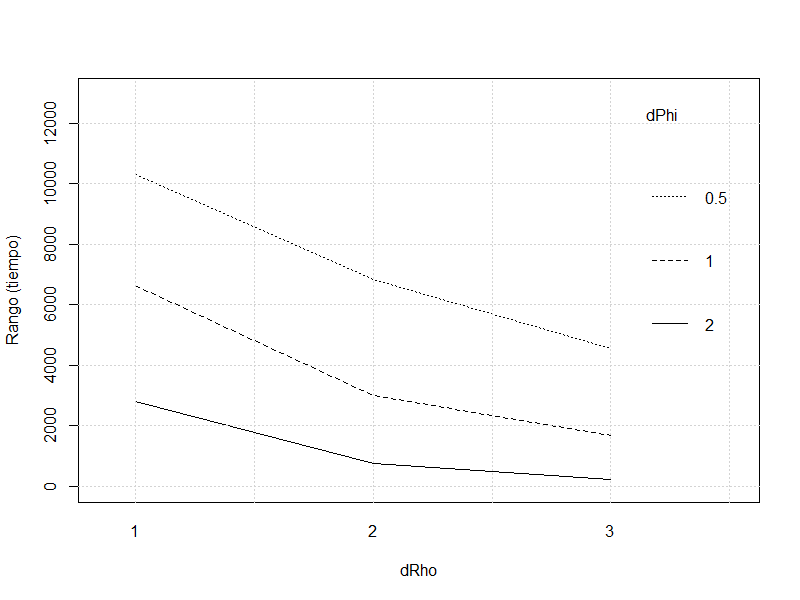
\includegraphics[width=0.5\textwidth]{images/t/t-3I-t3.png}
    }
\caption{Promedio de la interacción de tercer nivel para el experimento A.}
\label{tab:3I-A}
\end{figure}


%%%%%%%%%%%%%%%%%%%%%%%%%%%%%%%%%%%%%%%%%%%%%%%%%%%%%%%%%%%%%%%%%%%%%%%
%%%%%%%%%%%%%%%%%%%%%%%%%%%%%%%%%%%%%%%%%%%%%%%%%%%%%%%%%%%%%%%%%%%%%%%
%%%%%%%%%%%%%%%%%%%%%%%%%%%%%%%%%%%%%%%%%%%%%%%%%%%%%%%%%%%%%%%%%%%%%%%
%%%%%%%%%%%%%%%%%%%%%%%%%%%%%%%%%%%%%%%%%%%%%%%%%%%%%%%%%%%%%%%%%%%%%%%
%%%%%%%%%%%%%%%%%%%%%%%%%%%%%%%%%%%%%%%%%%%%%%%%%%%%%%%%%%%%%%%%%%%%%%%

\section{Experimento B}

\subsection{Verificación de supuestos}

Al igual que con el experimento A, se realizó una exploración visual que rechazó los supuestos de ANOVA, como se indica en la figura \ref{fig:sin-transformacion-p}. También se confirmó con la prueba de Lilliefors como lo demuestra la figura \ref{fig:lillie-p}; el estadístico calculado descarta normalidad, por lo que se prosiguió a aplicar transformaciones a los datos.

\begin{figure}[H]
    \centering
        \small{
        \begin{alltt}
        
        
            > lillie.test(data-p)
                Lilliefors (Kolmogorov-Smirnov) normality test
            data:  data-p
            D = 0.3546, p-value < 2.2e-16
        \end{alltt}
        }
    \caption{Prueba de Lilliefors para normalidad en R. El estadístico es mayor que el valor-p por lo que los datos no son normales.}
    \label{fig:lillie-p}
\end{figure}

\begin{figure}[H]
    \centering
    \subfigure[Cuantiles contra Cuantiles.]{
        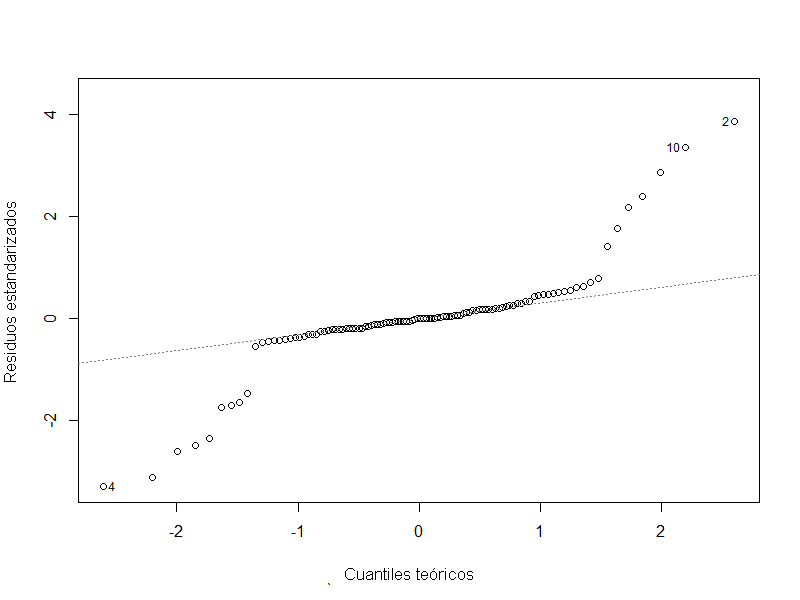
\includegraphics[width=.75\textwidth]{images/p/qq-p.png}
    }
    \subfigure[Residuos contra Valores Ajustados.]{
        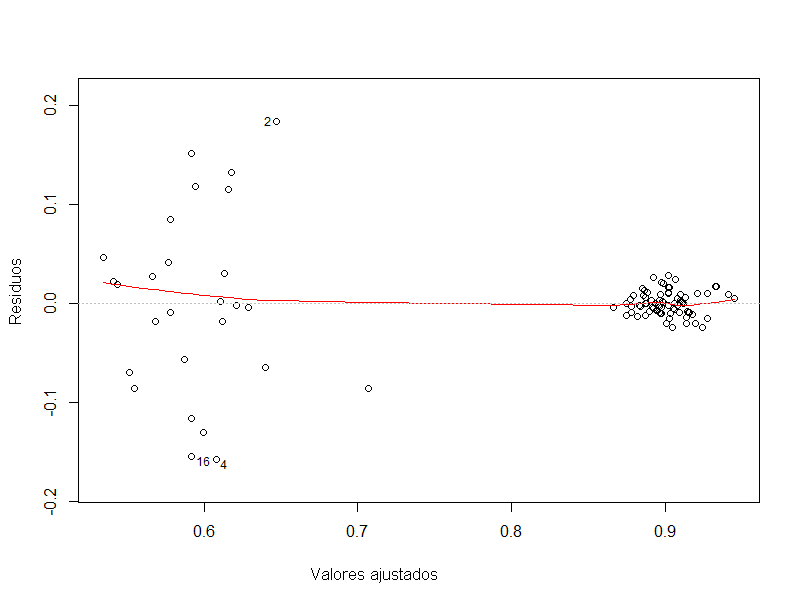
\includegraphics[width=.75\textwidth]{images/p/rvf-p.png}
    }
    \caption{Exploración visual de la normalidad y homogeneidad de varianza en los datos de precisión.}
    \label{fig:sin-transformacion-p}
\end{figure}

\subsubsection{Transformaciones}

Las transformaciones aplicadas a los datos de tiempo fueron aplicadas a los datos de precisión: potencia $e$, raíz cuadrada y logaritmo base 10.

En todos los casos, los supuestos fueron rechazados. Para cada transformación, potencia $e$, raíz cuadrada y logaritmo base 10, se muestran los gráficos Q-Q y RvAF, respectivamente en las figuras \ref{fig:transformacion-e-p} \ref{fig:transformacion-log-p} \ref{fig:transformacion-sqrt-p}.


\begin{figure}[H]
\centering
    \subfigure[Cuantiles contra Cuantiles de la Transformación con potencia $e$.]{
        \centering
        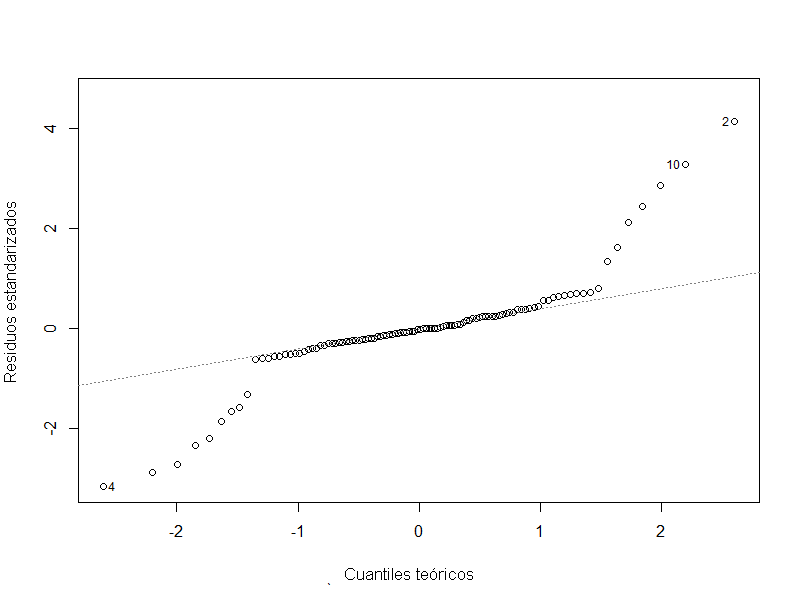
\includegraphics[width=0.75\textwidth]{images/p/qq-e.png}
    }
    \subfigure[Residuos contra Valores Ajustados de la Transformación con potencia $e$.]{
        \centering
        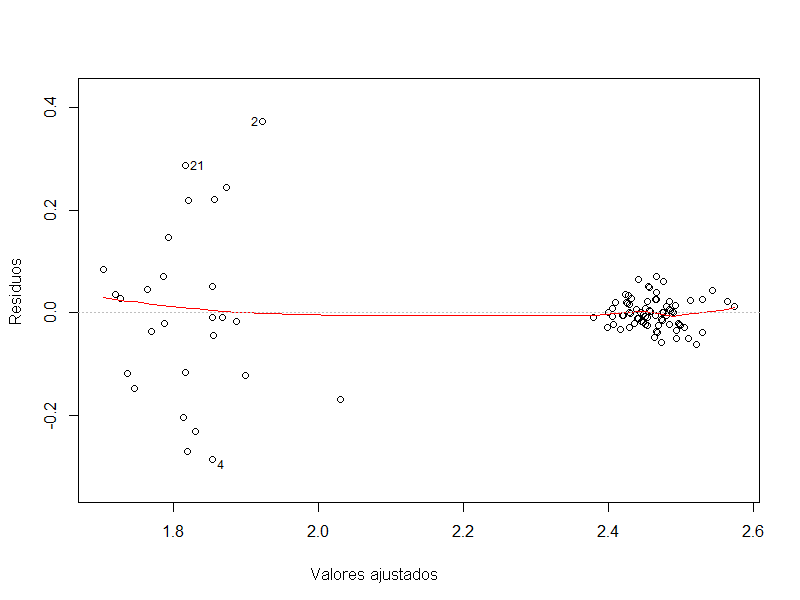
\includegraphics[width=0.75\textwidth]{images/p/rvf-e.png}
    }
\caption{Exploración visual de la normalidad y homogeneidad de varianza en los datos de precisión transformados con una potencia $e$.}
\label{fig:transformacion-e-p}
\end{figure}


\begin{figure}[H]
\centering
    \subfigure[Cuantiles contra Cuantiles de la Transformación con logaritmo base 10.]{
        \centering
        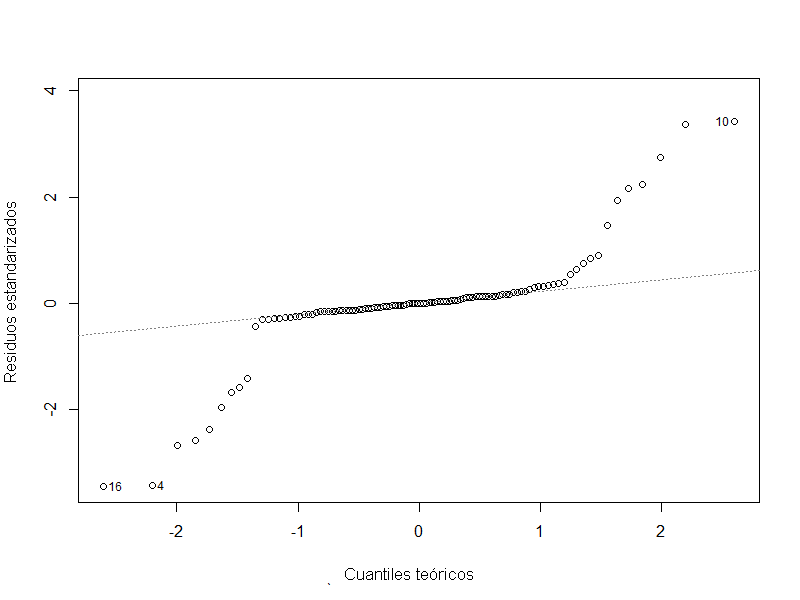
\includegraphics[width=0.75\textwidth]{images/p/qq-log.png}
    }
    \subfigure[Residuos contra Valores Ajustados de la Transformación con logaritmo base 10.]{
        \centering
        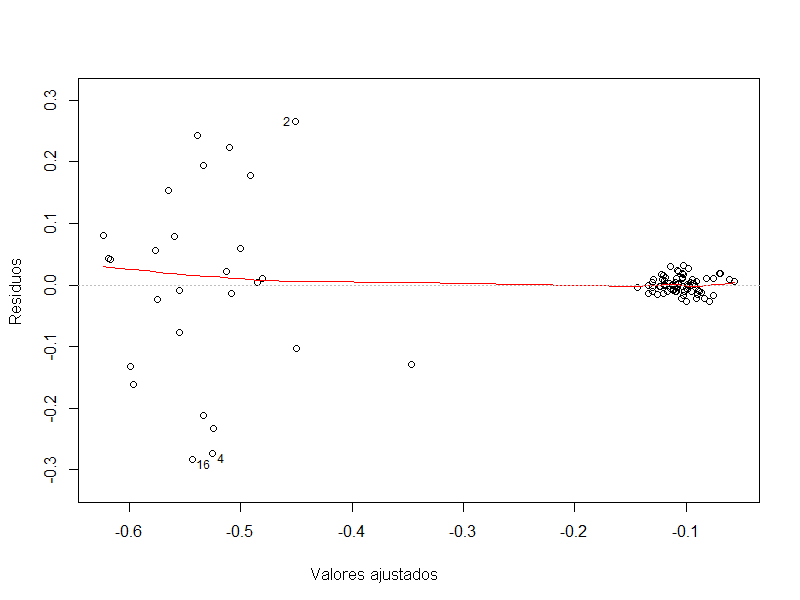
\includegraphics[width=0.75\textwidth]{images/p/rvf-log.png}
    }
\caption{Exploración visual de la normalidad y homogeneidad de varianza en los datos de precisión transformados con una logaritmo base 10.}
\label{fig:transformacion-log-p}
\end{figure}


\begin{figure}[H]
\centering
    \subfigure[Cuantiles contra Cuantiles de la Transformación con raíz cuadrada.]{
        \centering
        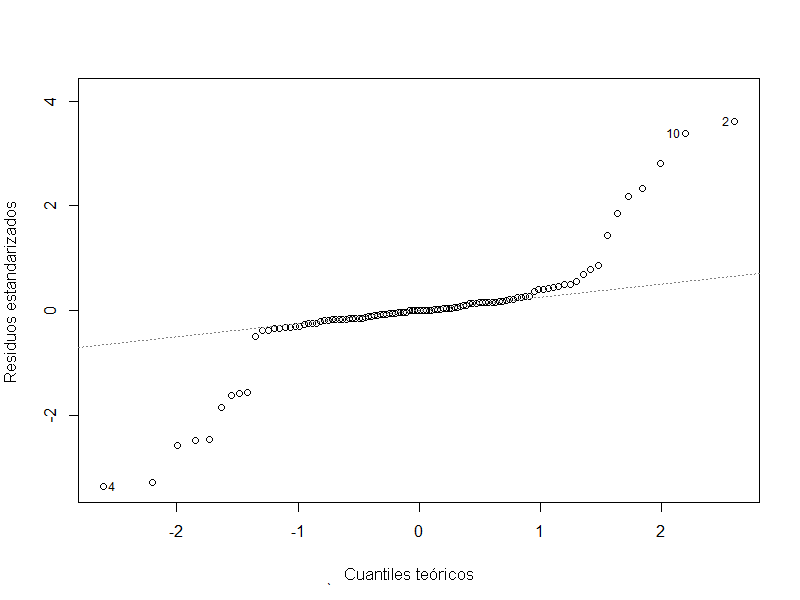
\includegraphics[width=0.75\textwidth]{images/p/qq-sqrt.png}
    }
    \subfigure[Residuos contra Valores Ajustados de la Transformación con raíz cuadrada.]{
        \centering
        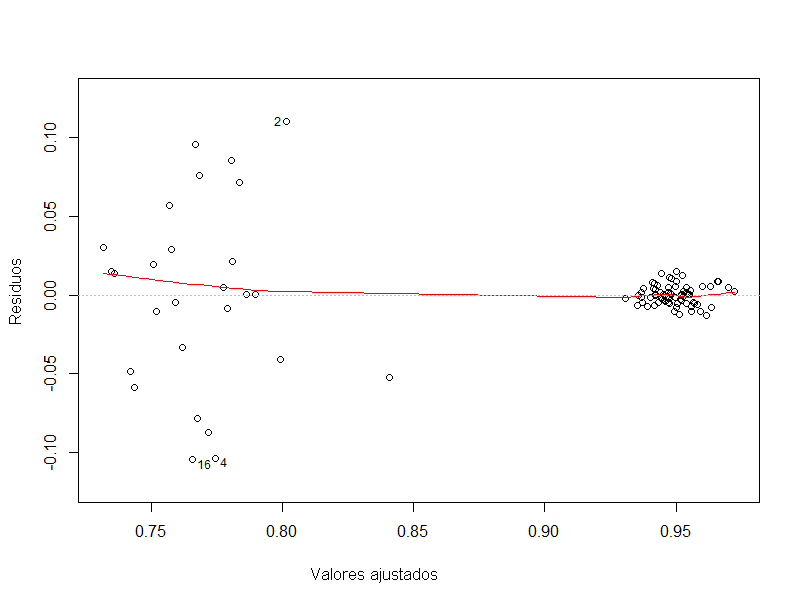
\includegraphics[width=0.75\textwidth]{images/p/rvf-sqrt.png}
    }
\caption{Exploración visual de la normalidad y homogeneidad de varianza en los datos de precisión transformados con una raíz cuadrada.}
\label{fig:transformacion-sqrt-p}
\end{figure}


\subsubsection{Modelo Lineal Generalizado}

El GLM fue descartado dadas las mismas razones que se plantean en el experimento A: no se pueden afirmar supuestos sobre distribución de errores de los datos de precisión ni establecer una función de enlace sin que sea de forma arbitraria.

Al igual que en el experimento A, se procedió a aplicar el método Box-Cox con la expectativa de que dicha transformación confirme los supuestos.

\subsubsection{Método Box-Cox}

El método Box-Cox reporta un valor $\lambda$ óptimo cerca de 2, como lo muestra la figura \ref{fig:box-cox-p}, por lo que se aplicó una transformación de potencia $2$ a los datos.

Infortunadamente la transformación rechaza los supuestos nuevamente. La figura \ref{fig:transformacion-bc-p} muestra la exploración visual que descarta normalidad y homogeneidad de varianzas.

\begin{figure}[H]
    \centering
    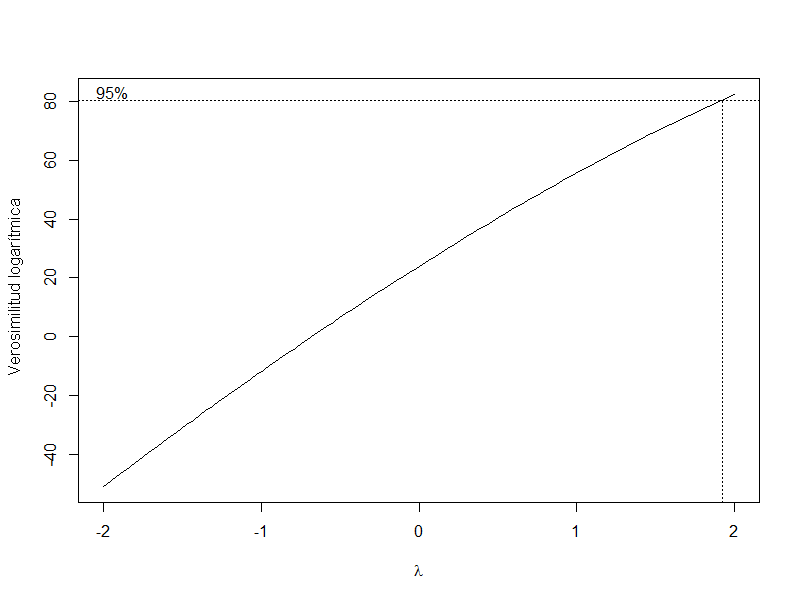
\includegraphics[width=0.75\textwidth]{images/p/box-cox-p.png}
    \caption{Método Box-Cox. El punto óptimo $\lambda$, con un 95\% de confianza se encuentra cerca de 2.}
    \label{fig:box-cox-p}
\end{figure}


\begin{figure}[H]
\centering
    \subfigure[Cuantiles contra Cuantiles de la Transformación con el método Box-Cox.]{
        \centering
        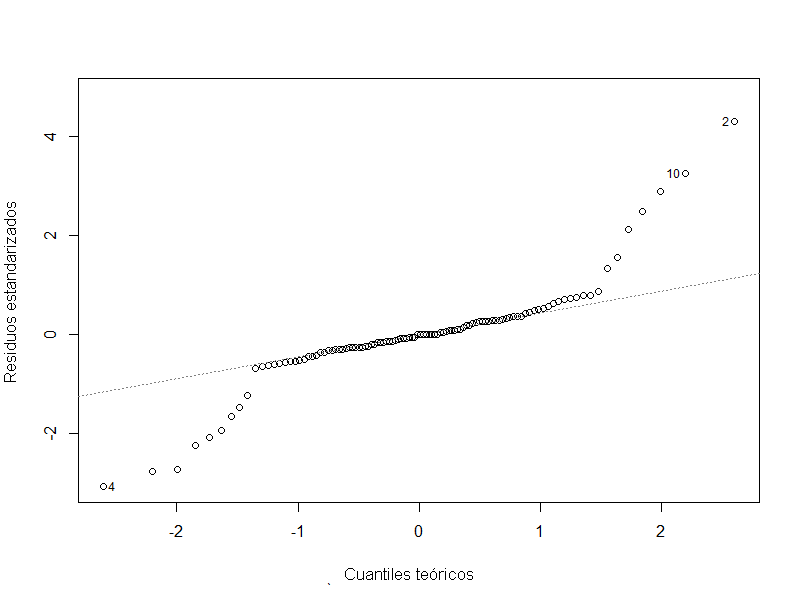
\includegraphics[width=0.75\textwidth]{images/p/qq-bc.png}
    }
    \subfigure[Residuos contra Valores Ajustados de la Transformación con el método Box-Cox.]{
        \centering
        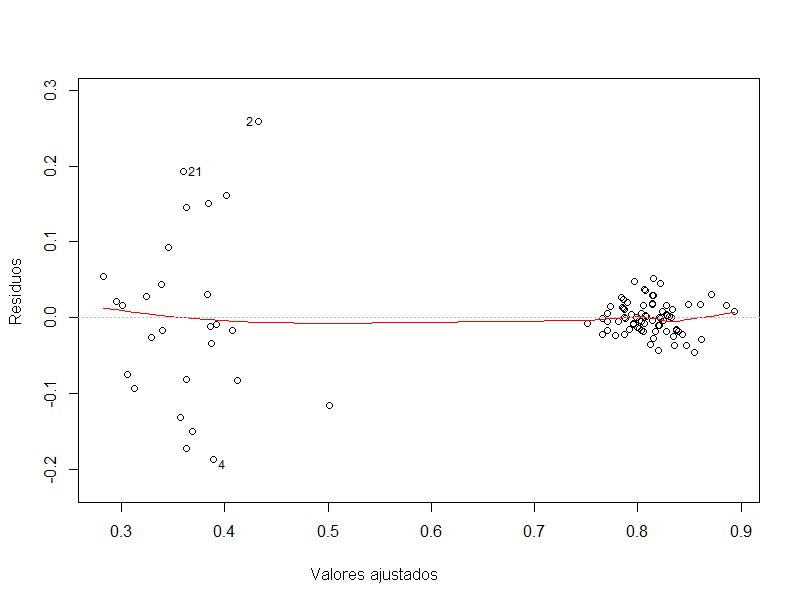
\includegraphics[width=0.75\textwidth]{images/p/rvf-bc.png}
    }
\caption{Exploración visual de la normalidad y homogeneidad de varianza en los datos de precisión transformados con el método Box-Cox.}
\label{fig:transformacion-bc-p}
\end{figure}

Dados estos fallos al verificar los supuestos, se optó por la misma solución que en el experimento A y aplicar una transformación por rangos.


\subsubsection{Transformación por Rangos}

Se aplicó en este caso una transformación por rangos donde un rango bajo significa una mala precisión, y un rango alto, una buena precisión (inverso al caso de los tiempos).

Así la peor precisión de 0,4375 tendrá el rango 1 y la mejor precisión 0,95 tendrá el rango más alto 212,5. Esta transformación se puede ver en la figura \ref{fig:rank-p}.


\begin{figure}[H]
    \centering
    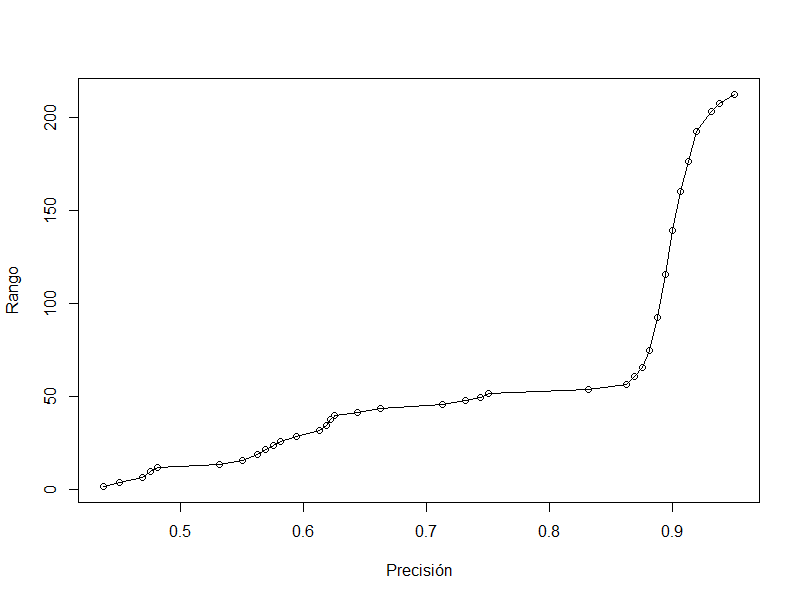
\includegraphics[width=0.75\textwidth]{images/p/rank.png}
    \caption{Transformación por rangos de los datos de precisión tomados en el experimento B.}
    \label{fig:rank-p}
\end{figure}


\subsection{Análisis de Resultados}

La tabla ANOVA se muestra en la figura \ref{tab:anovaB}.
Es preciso recordar que para este experimento, la transformación de los datos hizo que un rango bajo signifique una precisión alta (se puede ver también como el error en la clasificación).



\begin{table}\renewcommand{\tabcolsep}{3pt}
    \centering
    \small
    \begin{tabular}{lrrrrrr}
        \hline 
        Factor & Df & Sum Sq & Mean Sq & F-value & Pr($>$F) & Sig.\\
        \hline 
        \textbf{dTau} & 1 & 1168 & 1168 & 4.622 & 0.034752 & 0.05\\
        dPhi & 1 & 89 & 89 & 0.353 & 0.553947 &\\
        dRho & 1 & 133 & 133 & 0.528 & 0.469773 &\\
        \textbf{clasificador} & 3 & 72454 & 24151 & 95.560 & $<$2e-16 & 0\\
        dTau:dPhi & 1 & 58 & 58 & 0.230 & 0.632989 &\\
        dTau:dRho & 1 & 248 & 248 & 0.979 & 0.325495 &\\
        dPhi:dRho & 1 & 0 & 0 & 0.000 & 0.989759 &\\
        \textbf{dTau:clasificador} & 3 & 5793 & 1931 & 7.641 & 0.000157 & 0\\
        dPhi:clasificador & 3 & 1384 & 461 & 1.825 & 0.149661 &\\
        dRho:clasificador & 3 & 1970 & 657 & 2.598 & 0.058362 & 0.1\\
        dTau:dPhi:dRho & 1 & 462 & 462 & 1.827 & 0.180523 & \\
        dTau:dPhi:clasificador & 3 & 664 & 221 & 0.876 & 0.457247 & \\
        dTau:dRho:clasificador & 3 & 62 & 21 & 0.082 & 0.969620 & \\
        dPhi:dRho:clasificador & 3 & 208 & 69 & 0.275 & 0.843459 & \\
        dTau:dPhi:dRho:clasificador & 3 & 474 & 158 & 0.625 & 0.601146 & \\
        Residuals & 76 & 19208 & 253\\
        \hline
    \end{tabular}
    \caption{Tabla ANOVA para la precisión en la clasificación.}
    \label{tab:anovaB}    
\end{table}


Los factores e interacciones relevantes fueron: $\Delta \tau$, el clasificador y la interacción de segundo nivel entre ellos.

El factor $\Delta \tau$ presenta un efecto tenue sobre la variable de respuesta, sin importar su variación, la precisión se mantiene casi constante. La gráfica en la figura \ref{tab:ME-B} (a) muestra una línea prácticamente horizontal de $\Delta \tau$ contra los rangos de la precisión. 
Por otro lado la subfigura (b) muestra el tipo de clasificador contra los rangos. Aquí las diferencias son muy marcadas entre ellos. 
En promedio LogitBoost y SMO superan a los otros clasificadores, con rangos promedios de 163,64 (precisión de 0,9134259) y 142,90 (precisión de 0,9023148) respectivamente, y Kmeans es el peor de los cuatro con un rango promedio de 27,5 (tan solo 0,5952315 de precisión). 

\begin{figure}[H]
    \centering
    \subfigure[$\Delta \tau$]{
    
    	\includegraphics[width=0.75\textwidth]{images/p/p-MEdTau.png}
    }
    \subfigure[Clasificador]{
    
        \includegraphics[width=0.75\textwidth]{images/p/p-MEclasificador.png}
    }
\caption{Promedio del efecto de los factores $\Delta \tau$ y clasificador sobre la precisión.}
\label{tab:ME-B}
\end{figure}


La interacción de segundo nivel entre $\Delta \tau$ y el clasificador se puede apreciar en la figura \ref{tab:2I-B}. 
Aquí se puede notar claramente el gran peso que tiene el clasificador sobre la precisión, donde se pueden notar dos picos muy marcados, uno bajo en Kmeans y uno alto en LogitBoost. 
La diferencia entre cada uno de los clasificadores en términos de $\Delta \tau$ no es muy fuerte, especialmente con Kmeans. Se da un comportamiento interesante, en todos los clasificadores menos en Kmeans, donde la diferencia entre los promedios varía mucho con respecto a $\Delta \tau$.

\begin{figure}[H]

    \centering
	\includegraphics[width=0.75\textwidth]{images/p/p-2I.png}
\caption{Promedio de la interacción de segundo nivel entre $\Delta \tau$ y el clasificador para la precisión en el experimento B.}
\label{tab:2I-B}
\end{figure}

La figura \ref{fig:pix-p} grafica los clasificadores contra la cantidad de píxeles en promedio usados en cada configuración de parámetros de frecuencia.
La cantidad promedio de píxeles utilizada se calcula con la siguiente fórmula:

\begin{equation}
%(360/phi)*(len/rho)	((trazMax+trazMin)/2)*numTraz/tau
    \text{promedio píxeles} = \frac{trazMax + trazMin}{2} * \frac{numTraz}{\Delta \tau}
\end{equation}

Donde:
\begin{itemize}
    \item $trazMax$ es el trazo más largo que se puede hacer sobre la imagen, en este caso 500.
    \item $trazMin$ es el trazo más corto que se puede hacer sobre la imagen, en este caso 1.
    \item $numTraz$ es la cantidad de trazos que se hacen sobre la imagen según $\Delta \rho$ y $\Delta \phi$ y se calcula como se muestra a continuación:

    \begin{equation}
    %(360/phi)*(len/rho)	((trazMax+trazMin)/2)*numTraz/tau
        \text{numTraz} = \frac{360}{\Delta \phi} * \frac{trazMax}{\Delta \rho}
    \end{equation}
\end{itemize}


\begin{figure}[H]
    \centering
    	\includegraphics[width=1\textwidth]{images/p/pix-p.png}
\caption{Promedio del efecto de los factores $\Delta \tau$ y clasificador sobre la precisión.}
\label{fig:pix-p}
\end{figure}

En dicha figura se puede notar que, independientemente de la cantidad de píxeles utilizados para la extracción (por ende los parámetros de frecuencia), los clasificadores se comportan de manera similar y con poca variabilidad, con la excepción de Kmeans. LogitBoost oscila entre 0,88125 y 0,95, BayesNet entre 0,8625 y 0,9 y SMO entre 0,86875 y 0,93125.

\chapter{Conclusiones y trabajo futuro} 

A lo largo del presente trabajo se ha evaluado el desempeño de la Transformada de Trazo en términos de tiempo de extracción de características y precisión de clasificación. 

Los experimentos aquí realizados pretenden aportar evidencia estadística favor de la hipótesis de investigación:
\textit{La Transformada de Trazo presenta mejores resultados estadísticamente, en precisión de clasificación y en tiempo de extracción de características, al variar los parámetros de frecuencia, el tipo de clasificador y el tipo de cobertura.}
Se demostró estadísticamente como los parámetros de frecuencia influencian el tiempo de extracción y no así el tipo de cobertura de terreno. También se demostró como el clasificador utilizado afecta la precisión pero no así, todos los parámetros de frecuencia. 

A partir de los datos expuestos por los experimentos, se llega a las siguientes conclusiones:
\begin{enumerate}

\item A la luz del experimento A, \textbf{a parámetros de frecuencia más finos, mayor el tiempo de extracción}. La combinación de parámetros $\Delta \tau=1$, $\Delta \rho=1$ y $\Delta \phi=0.5$ resultan en el mayor tiempo de extracción y la combinación $\Delta \tau=3$, $\Delta \rho=3$ y $\Delta \phi=2$ en la menor.

\item De los parámetros de frecuencia, el que carga más peso para el tiempo de extracción es \textbf{$\Delta \tau$}: está presente en todas las interacciones reportadas como significativas. Esto hace que se necesite un particular cuidado al escoger este parámetro ya que los tiempos de respuesta pueden variar de 17,66167 a 52,60333 segundos en promedio.

\item El tipo de \textbf{cobertura} de terreno, a pesar de ser significativo estadísticamente cuando se transformó a rangos, \textbf{presenta mínimo efecto sobre el tiempo de extracción}.

\item El experimento B señala que \textbf{la precisión depende casi exclusivamente del clasificador utilizado}, donde el método aditivo LogitBoost presenta el mejor rendimiento.

\item De los parámetros de frecuencia, $\Delta \tau$ nuevamente se presenta como un factor relevante luego de transformar los datos a rangos, aunque en términos de \textbf{porcentaje de precisión la diferencia que hace escoger un valor u otro de $\Delta \tau$ es mínima}.

\item Según los datos experimentales, \textbf{no es útil hacer un barrido fino}. Los clasificadores se comportan de manera similar, a excepción de Kmeans, sea grueso o fino el barrido de la imagen. Las ganancias que pueden presentar los otros tres clasificadores, cerca del \textbf{7\% en precisión no justifica invertir 42 veces más tiempo en la extracción}. Aunque esta decisión tampoco debe tomarse a la ligera, pues depende del área de aplicación de la TT: tal vez en clasificación de imágenes áreas 7\% no sea de gran importancia, pero si las imágenes a procesar fueran de una tomografía axial computarizada para detectar cáncer, ese pequeño porcentaje podría salvar vidas.

\item Dados los tiempos y la precisión observada, es posible construir una versión de la TT que utilice valores gruesos de frecuencia y un clasificador LogitBoost que corra en un equipo portátil para giras de campo (geografía).

\end{enumerate}


\section{Aportes}

Dentro del alcance de esta propuesta se definen los siguientes entregables:
\begin{enumerate}
    \item Prototipo de un programa para la extracción de características usando la TT. En este prototipo deben ser parametrizables, los parámetros de frecuencia y el clasificador.
    \item Prototipo de los clasificadores.
    \item Programas auxiliares para la ejecución y el control de los 2 anteriores.
    \item Análisis estadístico para contrastar los resultados de los experimentos.
    \item Artículo científico que se entregará al comité editorial de alguna revista o conferencia, con miras a su publicación.
\end{enumerate}



El trabajo realizado en esta investigación cumplió con los entregables establecidos:
\begin{enumerate}
\item Una implementación de la TT parametrizada.
\item Una implementación de los clasificadores, utilizando el sistema Weka.
\item Los programas auxiliares para la ejecución y el control de los experimentos.
\item El análisis estadístico de los experimentos.
\item Un artículo científico, que fue aceptado para presentación y publicación en el IWOBI 2015\footnote{\url{http://iwobi.ulpgc.es/}}.
\end{enumerate}

\section{Trabajo futuro}
\label{sect:Future work}
Luego de realizar esta investigación surgen varias preguntas de investigación surgen y quedan abiertos varios caminos para plantear nuevos proyectos. Se proponen entonces las siguientes ideas para trabajos futuros:

\begin{enumerate}

\item Construir un generador de mapas de cobertura, utilizando la clasificación dada por el estudio aquí hecho y ajustado para maximizar la precisión y minimizar el tiempo de extracción de características.

\item Dadas las diferentes arquitecturas de procesadores y jerarquías de memoria, la medición y adaptación de la TT a otras plataformas de ejecución sería de interés para optimización.

\item La aplicación en imágenes más grandes y en otros campos, especialmente en las ciencias médicas, es de gran interés; existe un gran conjunto de datos de imágenes médicas que se puede explotar y que pueden tener un gran impacto en la calidad de vida.

\item El uso de una ventana de análisis en imágenes grandes se debe estudiar también, y contrastar con la técnica de segmentar la imagen en otras más pequeñas. Se puede a su vez medir el impacto que puede tener ésta ventana en la precisión.

\item La selección de funcionales y por lo tanto de TF es un tema que se debe abordar. Es posible que el aporte que brindan las TF no sea el mismo para la clasificación, y que un número mejor de funcionales sea posible de implementar sin perder precisión.

\item Se debe comparar el rendimiento de la TT contra otras técnicas automatizadas de clasificación de imágenes, particularmente en el área geográfica.
\end{enumerate}



% Appendixes
%\appendix 
%\input{Body/appendix1}

% Final pages
\backmatter

% Use single space
\singlespacing

% Bibliography
\cleardoublepage

\refstepcounter{chapter}

\addcontentsline{toc}{chapter}{\bibname}
\bibliography{common/references.bib}

\end{document}
